%% LyX 1.6.9 created this file.  For more info, see http://www.lyx.org/.
%% Do not edit unless you really know what you are doing.
\documentclass[oneside,english]{amsart}
%\documentclass[oneside,english]{article}
\usepackage[T1]{fontenc}
\usepackage[utf8]{inputenc}
\usepackage{amsmath,amssymb,graphicx}
\usepackage{amsthm}
\usepackage{graphicx}
\usepackage{siunitx}
%\usepackage{subfigure}
%\usepackage{epsfig}
%\usepackage{color}
%%%%%%%%%%%%%%%%%%%%%%%%%%%%%%%%%%%%%%%%%%%%%%%%
\graphicspath{{./Images/}}
%usepackage[dvips]{color}
%%%%%%%%%%%%%%%%%%%%%%%%%%%%%%%%%%%%%%%%%%%%%%%%%%%%%
\usepackage[left=2.5cm,right=2.5cm,top=3cm,bottom=3cm]{geometry}
%%%%%%%%%%%%%%%%%%%%%%%%%%%%%%%%%%%%%%%%%%%%%%%%%%%
%\newcommand{\cal}{\mathcal}
\newcommand{\beq}{\begin{equation}}
\newcommand{\eeq}{\end{equation}}
%%%%%%%%%%%%%%%%%%%%%%%%%%%%%%%%%%%%%%%%%%%%%%%%%%%%%
\def\sinc{\mathop{\rm sinc}\nolimits}  
\def\cal{\mathop{\rm cal}\nolimits}  
\def\cal{\mathop{\rm cal}\nolimits}  
\def\CFL{\mathop{\rm CFL}\nolimits}  
\def\ex{\mathop{\rm ex}\nolimits}  
\def\atan{\mathop{\rm atan}\nolimits}  
\def\sech{\mathop{\rm sech}\nolimits}  
\def\tanh{\mathop{\rm tanh}\nolimits}  
\def\div{\mathop{\rm div}\nolimits}  
\def\days{\mathop{\rm days}\nolimits}  
\def\Re{\mathop{\rm Re}\nolimits}  
\def\Sp{\mathop{\rm Sp}\nolimits}  
\newcommand{\bgrad}{\mbox{\boldmath$\nabla$}}
\newcommand{\bnabla}{\mbox{\boldmath$\nabla$}}
\newcommand{\bF}{\mbox{\boldmath$F$}}
\newcommand{\bP}{\mbox{\boldmath$P$}}
\newcommand{\bJ}{\mbox{\boldmath$J$}}
\newcommand{\bM}{\mbox{\boldmath$M$}}
\newcommand{\bg}{\mbox{\boldmath$g$}}
\newcommand{\bq}{\mbox{\boldmath$q$}}
\newcommand{\bx}{\mbox{\boldmath$x$}}
\newcommand{\bc}{\mbox{\boldmath$c$}}
\newcommand{\be}{\mbox{\boldmath$e$}}
\newcommand{\bn}{\mbox{\boldmath$n$}}
\newcommand{\bu}{\mbox{\boldmath$u$}}
\newcommand{\bv}{\mbox{\boldmath$v$}}
\newcommand{\bs}{\mbox{\boldmath$s$}}
\newcommand{\bi}{\mbox{\boldmath$i$}}
\newcommand{\bj}{\mbox{\boldmath$j$}}
%\newcommand{\bJ}{\mbox{\boldmath$J$}}
\newcommand{\bk}{\mbox{\boldmath$k$}}
\newcommand{\bvarphi}{\mbox{\boldmath$\varphi$}}
\newcommand{\bomega}{\mbox{\boldmath$\omega$}}
\newcommand{\bpsi}{\mbox{\boldmath$\psi$}}
%%%%%%%%%%%%%%%%%%%%%%%%%%%%%%%%%%%%%%%%%%%
\newcommand{\cJ}{\mbox{\mathcal{J}}}
%%%%%%%%%%%%%%%%%%%%%%%%%%%%%%%%%%%%%%%%%%%
 \newcommand{\fu}{\mathfrak{u}}
  \newcommand{\fv}{\mathfrak{v}}
  \newcommand{\fw}{\mathfrak{w}}
  \newcommand{\fz}{\mathfrak{z}}
  \newcommand{\fe}{\mathfrak{e}}
    \newcommand{\fr}{\mathfrak{r}}
    \newcommand{\fg}{\mathfrak{g}}
    \newcommand{\fq}{\mathfrak{q}}
%%%%%%%%%%%%%%%%%%%%%%%%%%%%%%%%%%%%%%%%%%%%%
% ** PERSONAL NEWTHEOREMS
\newtheorem{thm}{Theorem}[section]
\theoremstyle{definition}
\newtheorem{defi}[thm]{Definition}
\newtheorem{prop}[thm]{Proposition}
\theoremstyle{remark}
\newtheorem{remark}[thm]{Remark}

\def\gint{\displaystyle\int}


\makeatother

\usepackage{babel}

\begin{document}

\title{Numerical simulation of propagation problems on the sphere using a compact scheme}


\begin{abstract}
In this paper we continue the study of the compact scheme 
on the sphere introduced in 
\cite{Croisille-10, Croisille-12}. This scheme uses 
discrete differential operators on the Cubed Sphere. 
Considering propagation problems, the scheme is fully centered
and used a symmetric filter to eliminate high frequency
oscillating modes.
Numerical results on a broad series of numerical test cases
in climatology are presented, including
linear convection problems, the linearized shallow water 
and the non linear shallow water equations. 
These results demonstrate the
potential of the present approach 
in a variety of situations of interest accuracy and the 
stability of the present approach.
\end{abstract}

\author{M. Brachet and J.-P. Croisille\dag\ddag}
\address{\dag Universit\'e de Lorraine, D\'epartement de Math\'ematiques, F-57045 Metz, France\\
\ddag C.N.R.S., Institut Elie Cartan de Lorraine, UMR 7502, F-57045 Metz, France}
\email{matthieu.brachet@univ-lorraine.fr, jean-pierre.croisille@univ-lorraine.fr}

%%\date\today
\date{September 12, 2017}
\maketitle

{\sl Keywords: Cubed-Sphere grid - Compact finite difference scheme - 
Hermitian derivative - Vortex propagation}
%%%%%%%%%%%%%%%%%%%%%%%%%%%%%%%%%%%%%%%%%%%%%%%%%%%%%%%%%%%%%%%%%%%%
%%%%%%%%%%%%%%%%%%%%%%%%%%%%%%%%%%%%%
\section{Introduction}
\label{sec:1}
In this paper, we continue the development
of the compact scheme introduced in \cite{Croisille-10,Croisille-12}
for the numerical resolution of 
partial differential equations on the sphere.
We are interested in propagation equations in 
climatology (atmosphere and ocean), 
which are related in a way or another
to the spherical Shallow Water equations (SWE).
These equations represent the reference hyperbolic system
to be solved in spherical geometry. 
A second problem (LSWE) is the linearized (SWE) 
around an atmosphere at rest. On this problem and its importance
in climatology and oceanography,
we refer to the recent monograph\cite{Paldor} and the references
therein.

Equations SWE or LSWE on the sphere are the source of many efforts
to adapt conservative methods  
originating from numerical gas dynamics.
This is in particular the case of the finite volume
method \cite{Chen-Xiao, Ullrich-Jablonowski-vanLeer}.
or the Discontinuous Galerkin methods \cite{Bao-Nair-Tufo}.
Conservative methods 
are designed to be applied to the conservative form 
of the equations.
In the case of SWE, the vector height/momentum 
$q=[h,h\bv]$ is the vector of conservative variables. 
Such methods by construction
guarantee the conservation
of the components of the conservative vector $q$ over the full sphere. 
However additional quantities,
which are theoretically conserved by SWE,
such as  energy, potential enstrophy angular momentum
can suffer excessive dissipation.
The effective numerical conservation of 
these quantities for large time largely depends of the
built-in dissipation of the scheme. 

The numerical scheme we are considering here is a 
finite difference scheme
scheme over the Cubed Sphere grid. 
%It takes advantage of the specific structure
%of the Cubed Sphere, a grid widely used
%in the climatology community.
Aming the methods 
for fluid flows, this approach is related to 
the approximation of aeroacoustics equations by compact schemes,
along the lines of \cite{Lele, Visbal-Gaitonde, 
Tam-Webb, Bogey-Bailly}. This kind of approximation is also used
in the direct simulation of turbulence 
in parallelepipedic geometries \cite{Kim-Moin}.
Therefore our approach belongs to
a classical approach of computational fluid dynamics
which can be traced back to early works
in approximation and interpolation theory, \cite{Collatz}.
In the particular field of numerical climatology, 
it is related to \cite{Arakawa} and more recently
to the compact scheme presented in \cite{Ghader-Nordstrom}.
%%%%%%%%%%%%%%%%%%%%%%%%%%%%%%%%%%%%%%%%%%%%%%%%%%%%%%%%%%
The convective problems considered here 
are of three types.
\begin{itemize}
\item 
The linear scalar advection equation 
\begin{equation}
\label{eq:adv}
\dfrac{\partial h}{\partial t}  (t,\mathbf{x})+ \mathbf{c}(t,\mathbf{x}) 
\cdot \nabla_T h(t,\mathbf{x})=0
\end{equation}
In (\ref{eq:adv}), the velocity 
$\mathbf{c} : (t,\mathbf{x}) \in (0, +\infty) \times \mathbb{S}^2 \mapsto \mathbf{c}(t,\mathbf{x}) \in \mathbb{T}\mathbb{S}^2$ 
is prescribed so that the scalar value $h(t,\mathbf{x})$ 
exhibits two moving antipodal vortices \cite{Nair-Machenhauer,Nair-Jablonowski}.
This problem goes beyond the classical solid body rotation test case.
The analytical solution permits a sharp
evaluation and comparison of any numerical scheme
for (\ref{eq:adv}).
\item
The LSWE system around the atmosphere at rest $q_0=[H_0,\bv_0=\b0]$
with $H_0 >0$ a constant height, 
is expressed as:
\begin{equation}
\label{eq:lswe}
(LSWE) \left\{
\begin{array}{l}
\dfrac{\partial \eta}{\partial t} (t,\mathbf{x})+ H \nabla_T 
\cdot \mathbf{v}(t,\mathbf{x})=0\\
\dfrac{\partial \mathbf{v} }{\partial t} (t,\mathbf{x})+ 
g \nabla_T \eta(t,\mathbf{x}) + f(\mathbf{x}) \mathbf{k}(\mathbf{x}) \times
\mathbf{v}(t,\mathbf{x})=0\\
\end{array}
\right.
\end{equation}

The state at rest is 
$(h_0,\mathbf{v}_0)=(H,\b0)$ and the 
the 3-components unknowns is
the perturbation 
$(t,\mathbf{x}) \mapsto (\mathbf{v}(t,\mathbf{x}), \eta(t,\mathbf{x}))$.
\item The SWE system is nonlinear. Its vector form is:
\begin{equation}
\label{eq:swe}
(SWE) \left\lbrace
\begin{array}{l}
\dfrac{\partial h^{\star}}{\partial t} (t,\mathbf{x}) + \nabla_T \cdot \left( h^{\star}(t,\mathbf{x}) \mathbf{v}(t,\mathbf{x}) \right) =  0 \\
\dfrac{\partial \mathbf{v}}{\partial t}  (t,\mathbf{x}) + \nabla_T \left( \dfrac{1}{2} |\mathbf{v}(t,\mathbf{x})|^2 
+ g h(t,\mathbf{x}) \right) + \left( f(\mathbf{x}) + \zeta(t,\mathbf{x}) \right) \mathbf{n}(\mathbf{x}) \times \mathbf{v}(t,\mathbf{x}) =  \mathbf{0} 
\end{array}
\right.
\end{equation}
where $\zeta = \left( \nabla_T \times \mathbf{v} \right) \cdot \mathbf{n}$ 
is the {\it relative vorticity} and 
$h^{\star} = h - h_s$ with $h_s$ the bottom topography function.
\end{itemize}

The form (\ref{eq:swe}) is nonconservative. 
It is adopted here, mainly
due to the fact that the gradient term 
is attractive to handle numerically
compared to the conservative form, \cite{Bao-Nair-Tufo}.
Equations (\ref{eq:adv}), (\ref{eq:lswe}) and (\ref{eq:swe}) 
are used in many benchmark test cases in numerical climatology.

For these three convective models, 
we show that our centered scheme is numerically competitive 
compared to conservative upwind methods.
Since the scheme is not a priori conservative,
we show careful evaluation in time of the conserved quantities.

The outline of the paper is as follows.
In Section \ref{sec:2}, we recall the essential of 
our approach introduced in 
\cite{Croisille-10, Croisille-12}. In Section 
\ref{sec:3} several key aspects of 
our numerical scheme is presented with emphasis 
on the role of the filtering. 
In Section \ref{sec:4}, we present 
numerical results on a series of test cases
relevant for the three systems of equations above. 
% main focus
% is on the behaviour of the scheme
% in the wave or weakly nonlinear regime
% over the sphere.
% This dissipation
% must be kept as low as possible for realistic simulations.
% This can be difficult to achieve with FV or DG methods,
% because these additional conserved quantities are not part
% of the primal system of conserved unknows.
% Rather one simply observes how the method conserves them.


%%%%%%%%%%%%%%%%%%%%%%%%%%%%%%%%%%%%%%%%%%%% *** SECTION ***************************************************************************************************************

\section{Fourth order accurate spherical gradient}
\label{sec:2}
\subsection{Hermitian approach to partial derivatives on the sphere}
\label{sec:2.1}
In this section we present the principle
behind the calculation of the high-order accurate
approximate spherical gradient, as introduced in 
\cite{Croisille-10, Croisille-12}.
Consider a given function $ \mathbf{s} \in \mathbb{S}^2 \mapsto u(\mathbf{s})$ on the unit sphere
and a point $\bar{\mathbf{s}}$ where an approximate value of the tangential gradient
$\nabla_T u(\bar{\mathbf{s}})$ is required.
Consider a point $\mathbf{s}_0$ close to $\bar{\mathbf{s}}$ and two orthogonal great circles
$C_1$ and $C_2$ intersecting at $\mathbf{s}_0$. 
Denote by $\xi$ and $\eta$ the angles along $C_1$ and $C_2$ respectively.
The angles $(\xi,\eta)$ form a local coordinate system 
whose $\mathbf{s}_0(0,0)$ is the center. 
The tangential gradient $\nabla_T u(\bar{\mathbf{s}})$  is given by:
\beq
\label{eq:87.1}
\nabla_T u(\bar{\mathbf{s}})=
\Big(
\partial_\xi u(\bar{\mathbf{s}})
\Big)
g^\xi(\bar{\mathbf{s}})
+
\Big(
\partial_\eta u(\bar{\mathbf{s}})
\Big)
g^\eta(\bar{\mathbf{s}}).
\eeq
In (\ref{eq:87.1}), $(g^\xi(\mathbf{s}),g^\eta(\mathbf{s}))$
denotes the dual basis of the basis 
$(g_\xi(\mathbf{s}),g_\eta(\mathbf{s}))$ where
\beq
\label{eq:32.19}
g_\xi(\mathbf{s})=\frac{\partial \mathbf{s}}{\partial \xi},\;\;\;
g_\eta(\mathbf{s})=\frac{\partial \mathbf{s}}{\partial \eta}.
\eeq
Consider next the iso-$\eta$ curve passing through $\bar{\mathbf{s}}$.
This curve is locally defined as a function of the $\xi$ parameter as:
\beq
 \xi \in (\bar{\xi}-\varepsilon, \bar{\xi}+\varepsilon)
 \mapsto \mathbf{s}(\xi,\bar{\eta}), \;\;\; \varepsilon >0.
\eeq
Due to the orthogonality of the circles $C_1$ and $C_2$, this curve
is also an arc of great circle. We call $\bar{C}$ this great circle.
We define a discrete grid of $\bar{C}$ 
using the points with coordinates $\mathbf{s}_i(i\Delta \xi,\bar{\eta})$. The value
$\Delta \xi >0 $ is the constant step defined by
\beq
\Delta \xi = \frac{\pi}{2N}
\eeq 
and $N>0$ is an integer.
Assume for the moment that the point $\bar{\mathbf{s}}$ belongs to this grid and that 
$\bar{\mathbf{s}}=\mathbf{s}_i$ for some integer $i$.  A simple way 
to approximate $\nabla_T u(\bar{\mathbf{s}})$
is obtained by approximating in (\ref{eq:87.1}) 
the partial derivatives
$\partial_\xi u(\mathbf{s}_i)$ and $\partial_\eta u(\mathbf{s}_i)$.
Consider first $\partial_\xi u(\bar{\mathbf{s}})$.
Since $\bar{\mathbf{s}}=\mathbf{s}_i$, using 
the standard centered divided difference we have;
\beq
\label{eq:75.10}
\partial_\xi u(\mathbf{s}_i) \simeq 
\frac{u(\mathbf{s}_{i+1})- 
u(\mathbf{s}_{i-1})}{2 \Delta \xi}.
\eeq
The divided difference in the right-hand-side is denoted by $\delta_\xi u_i$.
Proceeding in the same manner in the $\eta$ direction, we set up
a grid on the circle $\bar{C}^\prime$:
the iso-$\xi$ great circle through by $\bar{\mathbf{s}}$ receives 
a grid with step size $\Delta \eta = \Delta_\xi$. The points
along this grid are numbered with index $j$ and we
call ${\mathbf{s}}=\mathbf{s}^\prime_j$. The value
$\partial_\eta u (\bar{s})$ is approximated by:
\beq
\label{eq:75.11}
\partial_\eta u(\bar{\mathbf{s}}) \simeq 
\delta_\eta u^\prime_j = \frac{u(\mathbf{s}^\prime_{j+1})- 
u(\mathbf{s}^\prime_{j-1})}{2 \Delta \eta}.
\eeq
A first candidate for the approximate value to $\nabla_T u(\bar{\mathbf{s}})$ is therefore:
\beq
\label{eq:87.2}
\nabla_{T,h} u(\bar{\mathbf{s}})=
\left(\delta_\xi u_i\right)
g^\xi(\bar{\mathbf{s}})
+
\left(\delta_\eta u^\prime_j \right)
g^\eta(\bar{\mathbf{s}}).
\eeq
The vector $\nabla_{T,h} u(\bar{\mathbf{s}})$ is obviously a second order 
approximation to $\nabla_T u(\bar{\mathbf{s}})$.
A simple way to go beyond second order
is to modifiy $\delta_\xi u_i$ using instead
the Hermitian derivative $\delta^H_\xi u_i$.
It is defined in terms of $\delta_\xi u_i$ by the relation
\beq
\label{eq:73.10}
\frac{1}{6} \delta_\xi^H u_{i-1}
+\frac{2}{3} \delta_\xi^H u_i
+\frac{1}{6} \delta_\xi^H u_{i+1}
= 
\delta_\xi u_i.
\eeq
The relation (\ref{eq:73.10}) defines implictely
$ \delta_\xi^H u_i$ as a perturbation of 
$\delta_\xi u_i$ since it can be expressed as:
\beq
\label{eq:73.14}
\delta_\xi^H u_i
= 
\delta_\xi u_i -\frac{\Delta^2\xi}{6} \delta^2_\xi \delta^H_\xi u_i
\eeq
The difference with (\ref{eq:75.10}) 
is that (\ref{eq:73.10}) involves values of $u$ along 
the full on $\bar{C}$ and not only the two neighboor values 
at $i\pm 1$.
Solving (\ref{eq:73.10}) provides $\delta^H u_i$.
This values satisfies the fourth-order consistency relation
\beq
\label{eq:34.18}
\delta^H_\xi u_i=
\partial_\xi u(\bar{\mathbf{s}})+ O(\Delta \xi^4)
\eeq
Proceeding in the same way along the $\eta-$ direction gives 
the approximation
\beq
\label{eq:34.19}
\delta^H_\eta u^\prime_j=
\partial_\eta u(\bar{\mathbf{s}})+ O(\Delta \xi^4)
\eeq
The Hermitian approximate gradient at the point $\bar{\bs}$ 
is therefore:
\beq
\label{eq:87.2.1}
\nabla^H_{T,h} u(\bar{\mathbf{s}})=
\left(\delta^H_\xi u_i\right)
g^\xi(\bar{\mathbf{s}})
+
\left(\delta^H_\eta u^\prime_j\right)
g^\eta(\bar{\mathbf{s}})
\eeq
It results from (\ref{eq:34.18}-\ref{eq:34.19}) that
$\nabla^H_{T,h} u(\bar{\mathbf{s}})$ satisfies the fourth order
consistency relation
\beq
\label{eq:87.4}
\nabla^H_{T,h} u(\bar{\mathbf{s}})=\nabla_{T} u(\bar{\mathbf{s}})+O(\Delta \xi^4)+O(\Delta \eta^4).
\eeq
The Hermitian approximation (\ref{eq:87.4}) is the basis of our approximate gradient on the Cubed-Sphere.
%%%%%%%%%%%%%%%%%%%%%%%%%%%%%%%%%%%%%%%%%%%%%%%%%%%%%%%%%%%%%%%%%%%%%%%%%%%
\subsection{Approximate gradient on the Cubed-Sphere}
%%%%%%%%%%%%%%%%%%%%%%%%%%%%%%%%%%%%%%%%%%%%%%%%%%%%%%%%%%%%%%%%%%%%%%%%%%%%
The Cubed Sphere is a grid of the sphere. This grid and variants were introduced by
various authors. A systematic
presentation was given in
\cite{Ronchi-Iacono-Paolucci}.
This grid has been widely used for numerical climatology.
The Cubed-Sphere is composed of six panels with
label $(k)=(I), (II), (II), (IV), (V)$ and $(VI)$. Each panel matches
the face of the cube, in which the sphere
is embedded. Each panel
supports a Cartesian grid of size $N\times N$.
It is equipped with a 
coordinate system $(\xi,\eta)$.
As in the preceding section,
$\xi$ and $\eta$ are angles along a couple of orthogonal great circles
intersecting at the center of the panel.
A typical panel and the associated grid is represented
on Fig. \ref{fig:1}.
The  grid points are called $\mathbf{s}_{i,j}^{(k)}$ with $ (I) \leq (k) \leq (VI)$ and
$ -N/2 \leq i,j \leq N/2$. 
In panel $(k)$ and for all fixed $j$, the points  $ i \mapsto \mathbf{s}_{i,j}$ are 
located along a great circle. This essential property of the Cubed-Sphere
permits to follow the idea presented in Section \ref{sec:2.1}: 
the calculation of an approximate gradient at $\mathbf{s}^{(k)}_{i,j}$
by mean of Hermitian derivatives.
The approximate gradient
$\nabla_{T,h} u^{(k)}_{i,j}$ is given by
\beq
\label{eq:85.13}
\nabla_{T,h} u^{(k)}_{i,j}=
u_{\xi,i,j}^{(k)} \mathbf{g}^{\xi, (k)}_{i,j} 
+
u_{\eta,i,j}^{(k)} \mathbf{g}^{\eta, (k)}_{i,j} 
\eeq
As in the preceding section, the values $ u_{\xi,i,j}^{(k)}$ and $u_{\eta,i,j}^{(k)}$
are Hermitian approximation of the partial derivatives $\partial_\xi u(\mathbf{s}^{(k)}_{i,j})$ and
$\partial_\eta u(\mathbf{s}^{(k)}_{i,j})$. The calculation of 
these Hermitian derivatives are
based on a set of data located along two great circles called $\bar{C}_{i,j}$ and $\bar{C}^\prime_{i,j}$.
The data along $\bar{C}_{i,j}$ and $\bar{C}^\prime_{i,j}$
are of course based on specific points of the Cubed-Sphere.
The choice of these points is detailed in \cite{Croisille-10, Croisille-12}
and we refer to these two references for more details.
Even if no mathematical proof is available yet, 
numerical evidence show a consistency close to $4$.
%%%%%%%%%%%%%%%%%%%%%%%%%%%%%%%%%%%%%%%%%%%%%%%%%%%%%%%%%%%%%%%%%%%%%%%%%%%%%%%%%
\begin{figure}
   \def\svgwidth{0.4 \textwidth}
\input{drawing13.pdf_tex}
\caption{The points of a typical panel of the Cubed-Sphere are classified in three categories:
(i) Circles correspond to {\sl internal} points; (ii) Squares correspond to {\sl edge} points ;
(iii) Pentagons correspond to {\sl corner} points}
\label{fig:1}
\end{figure}
\section{Central compact differencing 
on the Cubed Sphere}
\label{sec:2}
In this section, after a brief overview of 
the Cubed Sphere in Section
\ref{sec:CS}, the essential of
our central differencing approach using a compact scheme
is summarized in Section \ref{sec:2.1}.
In Section \ref{sec:2.2} a discrete counterpart 
of the operators gradient, divergence and curl
are deduced from this central differencing
is derived.
%%%%%%%%%%%%%%%%%%%%%%%%%%%%%%%%%%%%%%%%%%%%%%%%%%%%%%%%%%%%%%%%%%%%%%%%%%%
\subsection{The Cubed-Sphere}
%%%%%%%%%%%%%%%%%%%%%%%%%%%%%%%%%%%%%%%%%%%%%%%%%%%%%%%%%%%%%%%%%%%%%%%%%%%%
\label{sec:CS}
The Cubed Sphere is a grid of the sphere popular
in numerical climatology since \cite{Sadourny}.
A modern
presentation was given in
\cite{Ronchi-Iacono-Paolucci}.
This grid has been widely used for numerical climatology
in various contexts.
The Cubed-Sphere is composed of six panels ( six charts) 
labeled $(k)=(I), (II), (II), (IV), (V)$ and $(VI)$. Each panel 
can be considered as matching
the face of a cube. Each panel
supports a Cartesian grid of size $(N+1)\times (N+1)$.
It is equipped with a 
coordinate system $(\xi,\eta)$
whose coordinate lines are great circle sections. 
The angles $\xi$ and $\eta$ are identified as 
the two "equatorial" angles along a couple of orthogonal great circles
intersecting at the center of the panel. 
The Cubed Sphere is represented on Fig. \ref{fig:1}
and a typical panel is shown
on Fig. \ref{fig:2}.
The  only parameter of the Cubed Sphere is $N \geq 1$,
which denotes the number of cells in one direction on each panels. 
In the sequel, the points are denoted 
$\mathbf{s}_{i,j}^{(k)}$ with $ -N/2 \leq i,j \leq N/2$ and 
$ (I) \leq (k) \leq (VI)$ denotes the index of the panel.
Since our scheme is a finite difference scheme,
the discrete unknowns are attached to the points of the Cubed Sphere.
Therefore our scheme has $6 N^2 +2$ scalar unknowns evolving in time,
which is the total number of points on the Cubed Sphere.
%%%%%%%%%%%%%%%%%%%%%%%%%%%%%%%%%%%%%%%%%%%%%%%%%%%%%%%%%%%%%%%%%%%%%%%%%%%%%%%%%%%%%%%%%%%%%%%%%%%%
\subsection{Periodic compact differencing 
along great circles}
\label{sec:2.1}
%Equations (\ref{eq:adv}), (\ref{eq:lswe}) and (\ref{eq:swe}) require
%discrete tangential operators approximating
%the gradient, the divergence and the curl. 
%Our starting point is to perform 
%three point compact differencing along a series of 
%great circles on the Cubed Sphere.
%This principle is particularly suited 
%on the Cubed Sphere since on each panel,
%coordinate lines are sections of great circles.
%In addition, we take advantage of the periodic
%setting along these great circles.
%In particular, we avoid the definition of ghost points.
  
The simplest discrete compact operator is the fourth order discrete
differential which is now recalled.
Consider an equispaced grid with stepsize $\Delta x>0$ and data 
$u_j$ located at point $x_j=j\Delta x$. The centered finite difference on a regular grid 
with step $\Delta x$ is
\beq
\label{eq:87.13}
\delta_x u_j =\frac{u_{j+1}-u_{j-1}}{2 \Delta x}.
\eeq
Relation (\ref{eq:87.13}) is a second order approximation of the derivative
$u^\prime(x_j)$. Let $u(x)$ 
be a regular function and $u^\ast$ the gridfunction defined by
\beq
(u^\ast)_j=u(x_j).
\eeq
Then we have
\beq
\label{eq:87.14}
\delta_x u^\ast_j =u^\prime(x_j)+\frac{\Delta x^2}{12}
u^{(4)}(\xi_j),
\eeq
for a certain $\xi_j \in [x_{j-1}, x_{j+1}]$.
Consider now the {\it implicit relation} with unknown $\delta^H_x u_{j}$
\beq
\label{eq:73.10.27}
\frac{1}{6} \delta_\xi^H u_{j-1}
+\frac{2}{3} \delta_\xi^H u_j
+\frac{1}{6} \delta_\xi^H u_{j+1}
= 
\delta_\xi u_j.
\eeq
The relation (\ref{eq:73.10.27}) is a three point compact relation, 
meaning that the stencil of dependence 
consists of the three points is $x_{j-1},x_j,x_{j+1}$. 
In the periodic setting, 
$\delta_x^H u_j$ satisfies at each $j$ the consistency relation
\beq
\label{eq:87.14.1}
\delta^H_x u^\ast_j =u^\prime(x_j)
-\frac{\Delta x^4}{180}
u^{(6)}(\xi_j).
\eeq
for another $\xi_j \in [x_{j-1}, x_{j+1}]$, \cite{Lele, BenArtzi-Croisille-Fishelov-4}.
%%%%%%%%%%%%%%%%%%%%%%%%%%%%%%%%%%%%%%%%%%%%%%%%%%%%%%%%%%
\subsection{Hermitian gradient, divergence and curl operators}
%%%%%%%%%%%%%%%%%%%%%%%%%%%%%%%%%%%%%%%%%%%%%%%%%%%%%
\label{sec:2.2}
Equations (\ref{eq:adv}), (\ref{eq:lswe}) and (\ref{eq:swe}) require
discrete tangential operators approximating
the gradient, the divergence and the curl. 
Our starting point is to perform 
three point compact differencing along a series of 
great circles on the Cubed Sphere.
This principle is particularly suited 
on the Cubed Sphere since on each panel,
coordinate lines are sections of great circles.
In addition, we take advantage of the periodic
setting along these great circles.
In particular, we avoid the definition of ghost points.
As already mentioned, the fundamental of our scheme
is to evaluate Hermitian derivatives (\ref{eq:73.10.27}) 
along a series of great circles on the sphere.
These great circles are associated to
coordinates lines on each panel.
In a second time, discrete differential operators are
deduced from them.
Details can be found in \cite{Croisille-10, Croisille-12}.

On panel $(k)$, $(I) \leq (k) \leq (VI)$, the local basis is 
\beq
\label{eq:32.19}
\bg_\xi(\mathbf{x})=\frac{\partial \mathbf{x}}{\partial \xi},\;\;\;
\bg_\eta(\mathbf{x})=\frac{\partial \mathbf{x}}{\partial \eta}.
\eeq
and the dual basis is called $(\bg^\xi, \bg^\eta)$.
Let $\bx \in \mathbb{S}^2 \mapsto f(\bx)$ be a regular function.
The gradient is defined by
\beq
\nabla_T f= 
\partial_\xi f \bg^\xi +\partial_\eta f \bg^\eta
\eeq
Let $f^k_{i,j}$ 
be a given scalar gridfunction on the Cubed Sphere.
Denoting $h=\Delta \xi=\Delta \eta=\frac{\pi}{2N}$, we have
\beq
\label{eq:95.13}
\nabla_{T,h} f= 
 f_{\xi,i,j}^k (\bg^\xi)_{i,j}^k 
+
f_{\eta,i,j}^k (\bg^\eta)_{i,j}^k 
\eeq

Similarly if 
$\bv: \bx \in \mathbb{S}^2 \mapsto \mathbf{T}\mathbf{S}^2$
is a regular tangential vector field,
the divergence and curl are:
\beq
\label{eq:95.13.1}
\left\{
\begin{array}{l}
\nabla_T \cdot \bv= 
\partial_\xi \bv \cdot  \bg^\xi +\partial_\eta \bv \cdot \bg^\eta\\
\nabla_T \times \bv = 
\partial_\xi \bv \times \bg ^\xi +\partial_\eta \bv \times \bg ^\eta
\end{array}
\right.
\eeq
The discrete divergence and curl of 
a discrete tangential vector grid function
$\bv^k_{i,j}$ are called 
$\nabla_{T,h} \cdot \bv_{i,j}^k$ 
and $\nabla_{T,h} \times\bv_{i,j}^k$ respectively.
They are defined by
\beq
\left\{
\begin{array}{l}
\nabla_{T,h} \cdot (\bv)_{i,j}^k= 
(\bv)_{\xi,i,j}^k \cdot  (\bg^\xi)_{i,j}^k 
+
\nabla_{T,h}
(\bv)^k_{i,j} \cdot (\bg^\eta)^k_{i,j}\\
\nabla_{T,h} \times (\bv)_{i,j}^k = 
(\bv)_{i,j}^k \times (\bg ^\xi)^k_{i,j} 
+
(\bv)_{i,j}^k \times (\bg ^\eta)^k_{i,j}
\end{array}
\right.
\eeq
Due to (\ref{eq:87.14.1}), we expect these discrete operators
to be fourth order accurate.

\begin{prop}
If $f(\bx)$ and $\bv(\bx)$ are any given scalar (resp. tangential vector)
function on the sphere. If $f^\ast$ and $\bv^\ast$
are their restriction to the Cubed Sphere, then the
consistency relations hold:
\beq
\label{eq:11.91}
\begin{aligned}
\nabla_{T,h} f^k_{i,j}-(\nabla_T f)^{\ast,k}_{i,j}&=O (h^3)\\
\nabla_{T,h} \cdot \bv^k_{i,j}
-(\nabla_T \cdot  f)^{\ast,k}_{i,j}&=O (h^3)\\
\nabla_{T,h} \times \bv^k_{i,j}
-(\nabla_T \times  \bv)^{\ast,k}_{i,j}&=O (h^3)
\end{aligned}
\eeq
\end{prop}
\begin{proof}
Suppose that in relation (\ref{eq:87.14.1}) the data $f_j$ are perturbed
by a term of order $O(h^4)$. Then the resulting
perturbation of $f_\xi$ is at most of order $O(h^3)$.
The consistency error drops therefore from order $4$ to order $3$.
\end{proof}
%%%%%%%%%%%%%%%%%%%%%%%%%%%%%%%%%%%%%%%%%%%%%%%%%%%%%%%%%%%%%%%%%%%%%%%%%%%%%%%%%%%%%%%
\begin{figure}
\includegraphics[scale=0.4]{Images/fig6.jpg}
\caption{
The Cubed Sphere with grid parameter $N=16$.
The total number of gridpoints is $6 \times N^2+2=1538$ in this case.
The panels $(I)$, $(II)$, $(III)$ and $(IV)$ are located
around the equatorial plane $z=0$. The index of the north panel is $(V)$ 
and the one of the south panel is $(VI)$. 
}
\label{fig:1}
\end{figure}
%%%%%%%%%%%%%%%%%%%%%%%%%%%%%%%%%%%%%%%%%%%%%%%%%%%%%%%%%%%%%%%%%%%%%%%%
\begin{figure}
   \def\svgwidth{0.3 \textwidth}
\input{drawing13.pdf_tex}
\caption{
The points of a typical panel of the Cubed-Sphere are classified in three categories:
(i) Circles correspond to {\sl internal} points; (ii) Squares correspond to {\sl edge} points ;
(iii) Pentagons correspond to {\sl corner} points}
\label{fig:2}
\end{figure}
%%%%%%%%%%%%%%%%%%%%%%%%%%%%%%%%%%%%%%%%%%%%%%%%%%%%%%%%%%%%%%%%%%%%%
%%%%%%%%%%%%%%%%%%%%%%%%%%%%%%%%%%%%%%%%%%%%%%%%%%%%%%%%%%%%%%%%%%%%%%%
%%%% *** SECTION ***********************************************************************************************************************

\section{Centered compact scheme with filtering}
%%%%%%%%%%%%%%%%%%%%%%%%%%%%%%%%%%%%%%%%%%%%%%%%%%%%%%%%%%%%%%%%%%%%%%%%%%%%%%%%%%%%%%%%%%%
Our approximate scheme
uses a centered finite-difference approximation on the Cubed-Sphere.
In particular we do not use any kind of upwinding.
A stabilization mechanism is a linear filtering
at each time step. This kind of numerical 
algorithm is stronlgy related to so-called 
hyperviscous numerical diffusion.
%%%%%%%%%%%%%%%%%%%%%%%%%%%%%%%%%%%%%%%%%%%%%%%%%%%%%%%%%%%%%%%%%%%%%%%%%55
\subsection{Method of lines}
%%%%%%%%%%%%%%%%%%%%%%%%%%%%%%%%%%%%%%%%%%%%%%%%%%%%%%%%%%%%%%%%%%%%%%%%%%%%%%%%%%%%%%%%%%%
We consider the convection equation on the sphere
with tangential velocity 
$(\mathbf{x} ,t) \in \mathbb{S}^2 \times \mathbb{R}_+ \mapsto \mathbf{c}(\mathbf{x},t)$.
\beq
\label{eq:978.23.1}
\left\{
\begin{array}{l}
\partial_t h(\mathbf{x},t)+\mathbf{c}(\mathbf{x},t) \cdot \nabla_s h(\mathbf{x},t)=0,\\
h(\mathbf{x},0)=h_0(\mathbf{x}).
\end{array}
\right.
\eeq
Existence and uniqueness for (\ref{eq:978.23.1}) is
obtained by the method of characteristics.
The task is to calculate
an approximation of $h(\mathbf{x},t)$.

Let
$t \mapsto h^{(k)}_{i,j}(t)$ be a semidiscrete approximation
in space of (\ref{eq:978.23.1}). This semi-discrete 
approximation is 
the solution of the differential system:
\beq
\label{eq:978.23.1a}
\left\{
\begin{array}{l}
{d h_{i,j}^k(t) \over dt} +\mathbf{c}^{(k)}_{i,j}(t)\cdot  \mathbf{\nabla} h h_{i,j}^k(t)=0,
\quad -M\leq i,j\leq M,\;\;\; I\leq k\leq VI,\\
h^{(k)}_{i,j}(0)=h_0(\mathbf{s}^{(k)}_{i,j})
\end{array}
\right.
\eeq
where $\mathbf{c}^{(k)}_{i,j}(t) \triangleq \mathbf{c}(\mathbf{s}^{(k)}_{i,j})(t)$.
Denote by $H(t) \triangleq  h^{(k)}_{i,j}(t)$ the gridfuntion
with components $h^{(k)}_{i,j}$. The equation (\ref{eq:978.23.1}) 
is expressed in vector form as:
\beq
\label{eq:71.10.3}
\frac{d}{dt}H(t)=J(t) H(t)
\eeq
where $J(t)$ is the matrix corresponding to
\beq
[J(t) H(t)]_{i,j}^{(k)} \triangleq 
-\bc^{(k)}_{i,j}(t)\cdot  \bgrad_{T,h} h_{i,j}^k(t).
\eeq
Since fourth order accuracy in space is expected, we proceed with 
the explicit in time RK 4 approxaimtion in time for
(\ref{eq:71.10.3}).
Let $\Delta t>0$ be a time-step. The RK4 time-scheme
is applied to (\ref{eq:71.10.3}).

\begin{equation}
\label{eq:300.41-1}
\left\{ 
\begin{array}{l}
K^{(0)} = J(t^n)H^{n}\\
K^{(1)} = J(t^{n+1/2})(H^{n}+\frac{1}{2}\Delta t K^{(0)})\\
K^{(2)} = J(t^{n+1/2})(H^{n}+\frac{1}{2}\Delta t K^{(1)})\\
K^{(3)} = J(t^{n+1})(H^{n}+\Delta t K^{(2)})\\
H^{n+1} = H^{n}
+\Delta t\Bigg(\frac{1}{6}K^{(0)}+\frac{1}{3}K^{(1)}
+\frac{1}{3}K^{(2)}+\frac{1}{6}K^{(3)}\Bigg).
\end{array}\right.
\end{equation}
%%%%%%%%%%%%%%%%%%%%%%%%%%%%%%%%%%%%%%%%%%%%%%%%%%%%%%%%%%%%%%%%%%%%%%%%%%%%%
\subsection{Dissipation and dispersion analysis}
Finite difference schemes are usually described
by their dissipation and dispersion properties. 
A customary analysis of this kind is the so called {\sl modified equation}
analysis, \cite{Shokin}.  This analysis is usually 
performed on the linear advection equation
\beq
\partial_t u + c \partial_x u=0
\eeq
We recall next the main features of this analysis.
Consider a numerical scheme
\beq
\label{eq:76.10}
\frac{u^{n+1}_j-u^n_j}{\Delta t}
+ L_h u|^n_j =0
\eeq
In (\ref{eq:76.10}), the operator $L_h u^n_j$ approximates $-c \partial_x u$.
In operator form, the scheme (\ref{eq:76.10}) is rewritten as
\beq
\label{eq:56.10}
\frac{e^{\Delta t \partial_t}-1}{\Delta t} u^n_j = -L_h u|^n_j
\eeq
The Logarithm series provides the formal expansion 
\beq
\label{eq:87.12}
\partial_t = \frac{e^{\Delta t \partial_t}-1}{\Delta t}
-\frac{\Delta t}{2}\left(\frac{e^{\Delta t \partial_t}-1}{\Delta t}\right)^2
+\frac{\Delta t}{3}\left(\frac{e^{\Delta t \partial_t}-1}{\Delta t}\right)^3
-\frac{\Delta t}{4}\left(\frac{e^{\Delta t \partial_t}-1}{\Delta t}\right)^4
+....
\eeq
Using (\ref{eq:56.10}) in the right hand side of (\ref{eq:87.12}),
we obtain an identity of the form
\beq
\label{eq:34.13}
\partial_t u+ c \partial_x u=c \Big[
  E_1 h \partial_x^{(2)}u 
+ E_2 h^2 \partial_x^{(3)}u 
+ E_3 h^3 \partial_x^{(4)}u 
+ E_4 h^4 \partial_x^{(5)}u 
+...
\Big]
\eeq
This identity is called the modified equation of the scheme. It represents a transport equation
with a perturbation in the form of an asymptotic expansion
in powers of $h$. The coefficients $E_\alpha$ depends
only the Courant number $\lambda= c \Delta t /h$. 
In the case of the scheme (), the modifed equation 
is expressed as:
\beq
\partial_t u+ c \partial_x u=c\Big[ \frac{h^4}{360}(3 \lambda^4+2) \partial_x^{(5)}u
+ \sum_\alpha h^{\alpha}E_\alpha \partial_x^{(\alpha+1)}u
\eeq
The first coefficients are 
\beq
\label{eq:72.10}
\left\{
\begin{array}{l}
E_4= \frac{1}{360}(3 \lambda^4+2)\\
E_5= \frac{1}{144}\lambda^5\\
E_6= \frac{1}{3024}(-2+9\lambda^6)\\
E_7= \frac{1}{1152}\lambda^7\\
E_8= \frac{1}{25920}(\lambda^4-1)(5 \lambda^4-1)\\
E_9= -\frac{1}{4320}\lambda^5
\end{array}
\right.
\eeq
As a result the scheme is $4-$order. In addition it is found to
be dissipative for the term in $\partial_x^{(6)}$ but antidissipative
with the terms in $\partial_x^{(8)}$ and  $\partial_x^{(10)}$.
%%%%%%%%%%%%%%%%%%%%%%%%%%%%%%%%%%%%%%%%%%%%%%%%%%%%%%%%%%%%%%%%%%%%%%%%%%%%%%%%%
\subsection{Tenth-order hyperviscosity}
%%%%%%%%%%%%%%%%%%%%%%%%%%%%%%%%%%%%%%%%%%%%%%%%%%%%%%%%%%%%%%%%%%%%%%%%%%%%%%
\label{sec:4}
As described in the previous section, stabilisation mechanism could be useful
to obtain a better stability profile. 
In such a situation a high-order filtering is added at each time step. 
Numerical practice showed
that a tenth-order filter from \cite{Visbal-Gaitonde} gives good results.
At each time step the value $H^{(n)}$ in (\ref{eq:300.41-1}) is replaced 
by $\mathcal{F} H^{(n)}$ where $\mathcal{F}$ is the filtering operator
acting on the gridfunctions defined by 
the composition of two one-dimensional filters along the $\xi$ and the $\eta$ directions on each panel:
\beq
\mathcal{F}=\mathcal{F}_\xi \circ \mathcal{F}_{\eta}
\eeq
For a one-dimensional grid function $u_j$,
The filter $\mathcal{F}$ belongs to the class 
of the filters 
\beq
\label{eq:75.10.3}
\alpha_f u_{F,i-1}+
u_{F,i}+
\alpha_f u_{F,i+1}=
\sum_{^j=0}^J \frac{a_j}{2}(u_{i+j}+u_{i-j})
\eeq
This kind of filtering was originally introduced
in the Atmospheric Sciences community \cite{Alpert}.
The values of the coefficients in (\ref{eq:75.10}) are given
in \cite{Visbal-Gaitonde}. 
Our numerical results were performed 
with the explicit filter, corresponding to
$\alpha_f=0$ and to the coefficients:
\beq
\label{eq:978.25.3}
\left(
\begin{array}{c}
a_0\\
a_1\\
a_2\\
a_3\\
a_4\\
a_5
\end{array}
\right)
=
\left(
\begin{array}{c}
193/256\\
105/256\\
-15/64\\
45/512\\
-5/256\\
1/512
\end{array}
\right).
\eeq
The fact that () acts as a filter is reflected 
by the values of 
coefficients in (\ref{eq:72.10}) in the modified equation modified equation.
The term in $\partial_x^{(10)} u$ is now dissipative insted of being
antidissitaive without filter. It is now 
\beq
E_9= -\frac{1}{138240}\frac{32\lambda^6-135}{\lambda}
\eeq
All these results were obtained with MAPLE.

%%%%%%%%%%%%%%%%%%%%%%%%%%%%%%%%%%%%%%%%%%%%%%%%%%%%%%%%%%%%%%%%%%%%%%%%%%%%%%%%%%%%
%\section{Fourth order centered compact scheme 
%for the convection equation}
\section{Stability analysis in one dimension}
%%%%%%%%%%%%%%%%%%%%%%%%%%%%%%%%%%%%%%%%%%%%%%%%%%%%%%%%%%%%%%%%%%%%%%%%%%
In this section we present a convergence analysis 
of a fourth order difference scheme,
compact in space, and explicit in time.
Consider as a model problem the convection equation
\beq
\label{eq:18.12.1}
\partial_t u(x,t) + c \partial_x u=0, \;\; x \in \Omega=(0,L),\;\; t\geq 0,
\eeq
Periodic conditions are applied at $x=0$ and $x=L$.
The solution is $u(x,t)=u_0(x-ct)$. 
Our basic scheme for (\ref{eq:18.12.1})
consists in applying the method of lines
to (\ref{eq:18.12.1}) and to use the two following approximations: 
\begin{itemize}
\item
The spatial derivative $\partial_x u(t,x)$ is approximated 
by (see (\ref{eq:73.10.27})):
\beq
\label{eq:55.10.4}
\partial_x u(t,x_j) 
\simeq
\delta^H_x u_j
\eeq
\item
The time derivative is approximated by the RK4 scheme 
(explicit fourth order Runge-Kutta) scheme. 
\end{itemize}
The resulting scheme is fourth order in space and time.
In this section we present an analysis of this scheme.
It is based on the fact that the discrete solutions,
both semi discrete and fully discrete,
are known explicitely in the periodic context.

Note that this scheme is used in many contexts, 
see for example \cite{}.

%%%%%%%%%%%%%%%%%%%%%%%%%%%%%%%%%%%%%%%%%%%%%%%%%%%%%%%%%%%%%%%
\subsection{Explicit discrete solution and stability analysis}
%%%%%%%%%%%%%%%%%%%%%%%%%%%%%%%%%%%%%%%%%%%%%%%%%%%%%%%%%%%%%
Proceeding along the method of lines, (\ref{eq:18.12.1}) 
is first approximated in space using (\ref{eq:55.10.4}), keeping the time continous. 
Let $x_j=jh$, with $h=L/N$, $N \geq 0$ be a finite difference grid
on the interval $\Omega$. 
Let $t \mapsto V(t)=[v_0(t),v_1(t),\dots v_{N-1}(t)]^T$ be the approximate value
of the exact solution 
$u^\ast(t)=[u(t,x_0),u(t,x_1),\dots,u(t,x_{N-1})]^T$.
The vector $V(t)$ is solution of the differential equation
\beq
\label{eq:71.10.3.4}
\frac{d}{dt}V(t)=-\frac{c}{h}\bJ V(t)
\eeq
The matrix $\bJ \in \Bbb C ^{N \times N}$ corresponds to the 
Hermitian derivative operator
\beq
u_j \mapsto \delta_x^H u_j.
\eeq
The discrete periocidity translates to the
relation
\beq
u_{j+\alpha N}(t)=u_j(t), \;\; \forall \alpha \in \Bbb Z, \;\; 0 \leq j \leq N-1.
\eeq
The solution of (\ref{eq:71.10.3.4}) is
\beq
V(t)= \exp\left(-\frac{c}{h}\bJ t \right)V_0
\eeq
where $V_0=[u_0(x_0),u_0(x_1), \dots, u_0(x_{N-1})]^T$.
The matrix $-\frac{c}{h}\bJ$ in the right-hand side 
is explicitely known, due to the fact
that $\bJ$ is expressed in terms of the matrix $\bP \in \Bbb R^{N \times N}$
\begin{equation}
\bP=\underbrace{\begin{pmatrix}
0&0&\cdots&0&1\\
1&\ddots&\ddots&\ddots&\vdots\\
\vdots&&\ddots&\ddots&0\\
0&&&\ddots&0\\
0&0&\cdots&1&0
\end{pmatrix}}_{N \times N}
\end{equation}
The matrix $\bP$ corresponds to the right shift operator
$ u_j \mapsto u_{j+1}$ with $N-$ periodic data.
Let $\omega=\exp(\frac{2 i \pi}{N})$.
For all $-N/2=1 \leq k \leq N/2$,
let $R^k=[R^k_0, R^k_1, \dots, R^k_{N-1}]^T \in \Bbb C^N$
be the vector with component $R^k_j$
\beq
R^k_j=\frac{1}{\sqrt{N}}\omega^{kj}, \;\;\; 0 \leq j \leq N-1.
\eeq
Notice that the vector $R^k$ satisfies
the relation
\beq
\bP R^k=\omega^k R^k.
\eeq
Therefore the vectors $R^k$ are eigenvectors
of $\bP$ associated to the eigenvalue $\omega^k$.
Since the $N$ complex numbers $\omega^k$ are all distincts,
they are {\sl all} the eigenvalues of the matrix $\bP$.
Furthermore, the vectors $R^k$ form
an orthogonal basis of $\Bbb C^N$ and due to the scaling constant 
$\frac{1}{\sqrt{N}}$, this basis is in fact orthonormal.
Consequently, the matrix $\bP$ is diagonalizable and it
can be expressed in spectral
form as
\beq
\bP= \sum_{k=-\frac{N}{2}+1}^{\frac{N}{2}} \omega^k R^k \otimes (R^k)^T
\eeq
where $\otimes$ denotes the Kronecker product. 
Due to the definition (\ref{eq:73.10.27}) of the Hermitian derivative, 
the matrix $\bJ$ is expressed in terms
of $\bP$ as
\beq
\label{eq:76.01.3}
\bJ=m(\bP),
\eeq
where $m(z)$ is the rational fraction
\beq
m(z)=\frac{1}{2}\frac{z-z^{-1}}{\frac{1}{6}(z+z^{-1})+\frac{2}{3}}.
\eeq
The eigenvalues of $\bJ$ are therefore the complex numbers 
$\mu_k=m(\lambda_k)$
 and the spectral decomposition of $\bJ$ is
\beq
\label{eq:74.10}
\bJ= \sum_{k=-\frac{N}{2}+1}^{\frac{N}{2}} m(\omega^k) R^k \otimes (R^k)^T.
\eeq
Noting that the eigenvalues of the scaled matrix $ -\frac{c}{h} \bJ$ 
in (\ref{eq:71.10.3.4}) are
the numbers $-\frac{c}{h} m(\omega^k)$ where $
-\frac{N}{2}+1 \leq k \leq  \frac{N}{2} $, the 
solution $V(t)$ of (\ref{}) is therefore 
expressed as 
\beq
\label{eq:13.12}
V(t)=\sum_{k=-\frac{N}{2}+1}^{\frac{N}{2}} 
\exp\left(-\frac{c}{h}m(\omega^k)t\right) \left((R^k)^T V_0\right) R^k
\eeq
Here we can compare $V(t)$ and the exact solution
$U(t)=[u(t,x_0), u(t,x_1), \dots,u(t,x_{N-1})]^T $.



\begin{prop}
The error $e_j(t)=u(t,x_j)-v_j(t)$ satisfies
\beq
\vert e_j(t) \vert \leq C(t) h^4,\; j=0,1,\dots,N-1
\eeq
\end{prop}
\begin{proof}
The exact solution is $u(t,x_j)=u_0(x_j-ct)$ is given in Fourier series by (we note $\tilde k =2 \pi k/L$):
\beq
\label{eq:91.10}
u(t,x_j)=\sum_{k \in \Bbb Z} \exp(i\tilde k(x_j-ct))\hat{u}_0^k
\eeq
where
\beq
\hat{u}_0^k=\frac{1}{\sqrt{L}}\int_0^{L} u_0(x)\exp(-i \tilde{k} x) dx
\eeq
We compare (\ref{}) and (\ref{}) at $x_j$ (....)
\end{proof}




















%%%%%%%%%%%%%%%%%%%%%%%%%%%%%%%%%%%%%%%%%%

Consider now the time stepping of (\ref{eq:71.10.3.4}) by the RK4 scheme.
%For the ODE
%\beq
%\label{eq:71.10.3}
%\frac{d}{dt}U(t)=J(t) U(t)
%\eeq
%it reads
%\begin{equation}
%\label{eq:300.41.1}
%\left\{ 
%\begin{array}{l}
%K^{(0)} = cJ(t^n)U^{n}\\
%K^{(1)} = cJ(t^{n+1/2})(U^{n}+\frac{1}{2}\Delta t K^{(0)})\\
%K^{(2)} = cJ(t^{n+1/2})(U^{n}+\frac{1}{2}\Delta t K^{(1)})\\
%K^{(3)} = cJ(t^{n+1})(U^{n}+\Delta t K^{(2)})\\
%U^{n+1} = U^{n}
%+\Delta t\Bigg(\frac{1}{6}K^{(0)}+\frac{1}{3}K^{(1)}
%+\frac{1}{3}K^{(2)}+\frac{1}{6}K^{(3)}\Bigg).
%\end{array}\right.
%\end{equation}
Since the matrix $-\frac{c}{h} \bJ$ is constant,
this scheme coincides with the time 
vector iteration
\beq
V^{n+1}= r(-\lambda \bJ) V^n 
\eeq
where $\lambda=c \Delta t/h$ is the Courant number 
and $r(z)$ is the truncated exponential series 
to 4th order
\beq
r(z)=1+z+\frac{z^2}{2!}+\frac{z^3}{3!}+\frac{z^4}{4!}
\eeq
Using (\ref{eq:74.10}) yields
the following formula for $V^n$ 
\beq
\label{eq:48.42}
V^n=\sum_{k=-\frac{N}{2}+1}^{\frac{N}{2}} 
[r(-\lambda m(\omega^k))]^n \left((R^k)^T V_0\right) R^k
\eeq
%%%%% START MATTHIEU BRACHET %%%%%%%%%%%%%%%%%%%%%%%%%%%%%%%%%%%%%%%%%%%%%%%%%%%%%%%%%%%%%%%%%%%%
The scheme is stable if and only if :
\beq
\Sp (r(-\lambda J)) \subset \mathcal{B}(0,1)
\eeq
If $\mathcal{D}_{RK4}$ is the domain of stability
of the RK4 scheme indicated on Fig. \ref{fig:stab_rk4}.
The scheme (\ref{}) is stable under the condition
\beq
\label{eq:55.12}
\Sp (-\lambda J) \subset \mathcal{D}_{RK4}
\eeq

\begin{figure}[htbp]
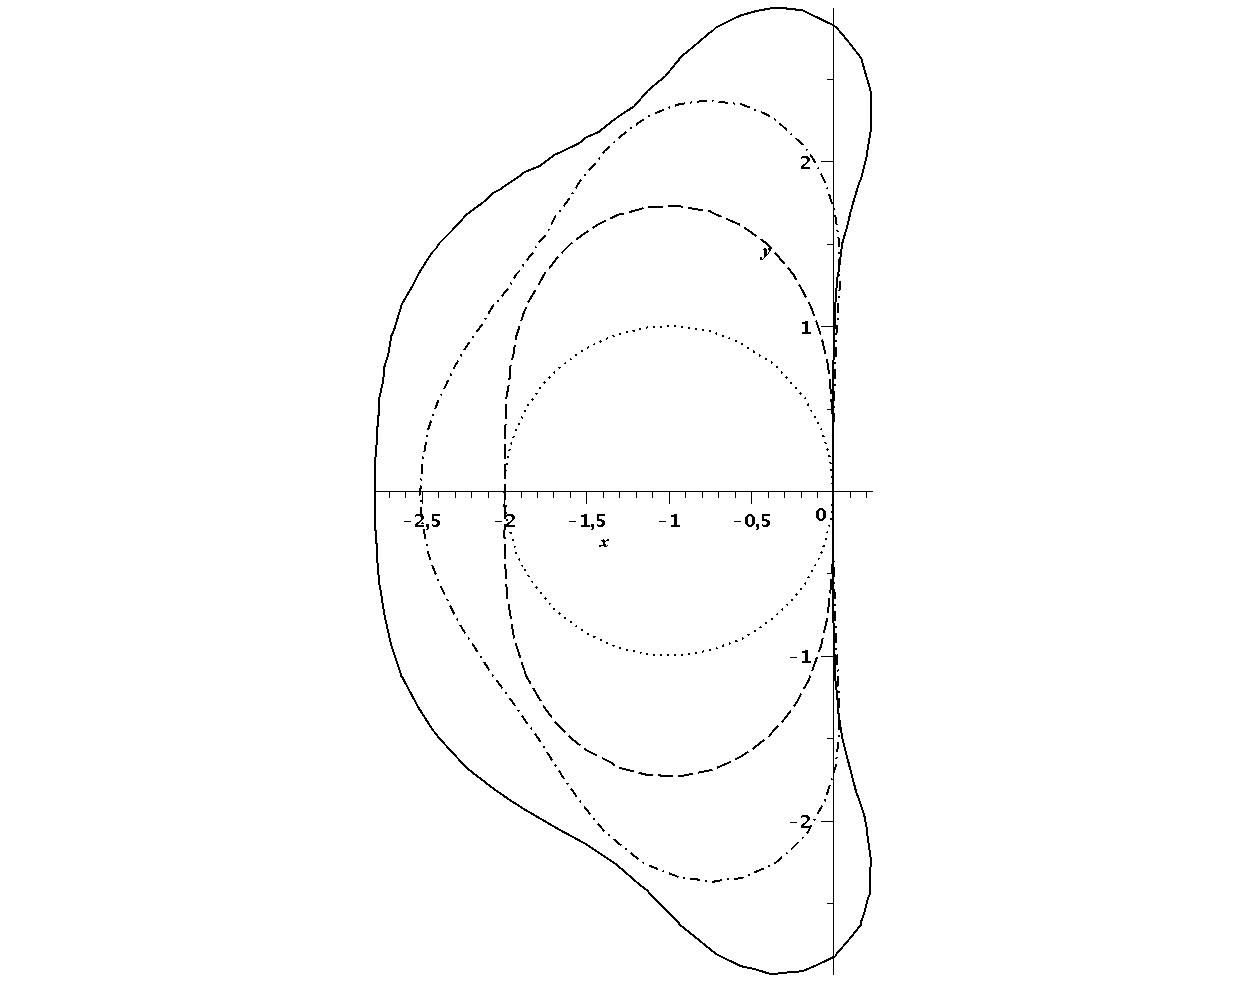
\includegraphics[scale=.2]{stabilityarea_NB.jpeg}
\caption{Domain of stability of the Backward Euler method (dotted point), Runge Kutta order 2 (dashed points), ordre 3 (mixed dotted and dashed points) and order 4 (continuous line) in the compex plan.}
\label{fig:stab_rk4}
\end{figure}

\begin{prop}
The condition (\ref{eq:55.12}) is satisfied
under the CFL condition
\beq
\lambda \leq \frac{K_{RK4}}{M} \simeq 1.62
\eeq
where $K_{RK4} \simeq 2.82 $ is the constant of the RK4 scheme
and $M$ is 
\beq
M= \max_{\theta  \in [0,\pi)}\left( \frac{\sin \theta}{\frac{2}{3}+\frac{1}{3}\cos \theta}
\right) = \sqrt{3}
\eeq
\end{prop}
\begin{proof}
The eigenvalues of $- \lambda \bJ$ are the numbers $- \lambda m(\omega_k)$ where $-\frac{N}{2}+1 \leq k \leq \frac{N}{2}$ :
\beq
- \lambda m(\omega_k) = - \lambda \dfrac{i \sin \left( \frac{2 k \pi}{N} \right)}{\frac{2}{3} + \frac{1}{3}\cos \left( \frac{2 k \pi}{N} \right)}
\eeq 
Then, the eigenvalues are on the imaginary axes. That implies the following result :
\beq 
Sp( - \lambda \bJ ) \subset \mathcal{D}_{RK4} \Rightarrow |- \lambda \dfrac{i \sin \left( \frac{2 k \pi}{N} \right)}{\frac{2}{3} + \frac{1}{3} \cos \left( \frac{2 k \pi}{N} \right)}| \leq K_{RK4} \text{ where } -\frac{N}{2}+1 \leq k \leq \frac{N}{2}.
\eeq

Then, because $\lambda > 0$, 
\beq
\lambda \leq \dfrac{K_{RK4}}{M}
\eeq

with $M=\max_{\theta  \in [0,\pi)}\left( \frac{\sin \theta}{\frac{2}{3}+\frac{1}{3}\cos \theta}
\right) = \sqrt{3}$ and the results is proved. 
\end{proof}


The convergence of the fully discrete scheme is given in
\begin{prop}



\end{prop}

%%%%%%%%%%%%%%%%%%%%%%%%%%%%%%%%%%
\subsection{Filtered time-scheme}
%%%%%%%%%%%%%%%%%%%%%%%%%%%%%%%%%%
Consider now the modified time scheme,
where a filtering step is added at the end of
each time step.
at the end of each time step (\ref{}) in the form
\beq
\label{eq:55.19}
U^{n+1} = \mathcal{F}\left(
U^{n}
+\Delta t\Bigg(\frac{1}{6}K^{(0)}+\frac{1}{3}K^{(1)}
+\frac{1}{3}K^{(2)}+\frac{1}{6}K^{(3)}\Bigg)
\right)
\eeq
The filter $\mathcal{F}$ is a linear operator
of the form \cite{Alpert}
\beq
\label{eq:75.10.3}
\alpha_f \mathcal{F}(u_{i-1})+
\mathcal{F}(u_{i})+
\alpha_f \mathcal{F}(u_{i+1})=
\sum_{j=0}^J \frac{a_j}{2}(u_{i+j}+u_{i-j})
\eeq
with the consistency condition
\beq
1+2 \alpha_f = \sum_{j=0}^J a_j
\eeq
Let $\beta(z)$ be the function associated with $\mathcal{F}$ 
given by
\beq
\beta(z)= \frac{\sum_{j=0}^J \frac{a_j}{2}(z^j+z^{-j})}{1 + \alpha (z+z^{-1})}
\eeq
The CFL stability condition becomes 
\beq
\label{eq:33.09}
\max_{\theta \in [0,\pi)}
\left(
\vert \beta(e^{i \theta}) \vert \vert r(-\lambda m(e^{i\theta})) \vert
\right)
\leq
1
\eeq
A sufficient condition on $\lambda$ for (\ref{eq:33.09}) is given by
\begin{prop}
\beq
\lambda \leq (...)
\eeq
\end{prop}



%%% END MATTHIEU BRACHET %%%%%%%%%%%%%%%%%%%%%%%%%%%%%%%%%%%%%%%%%%%%%%%%%%%%%%%%%%%%%%%%%%%%%%%%%%%%

%%%%%%%%%%%%%%%%%%%%%%%%%%%%%%%%%%%%%%%%%%%%%%%%%%%%%%%%%%%%%%%%%%%
\section{A centered scheme on the Cubed Sphere}
\label{sec:3}
%%%%%%%%%%%%%%%%%%%%%%%%%%%%%%%%%%%%%%%%%%%%%%%%%%%%%%%%%%%%%%%%%%%%%%%%%%%%%%%%%%%%%%%%%%%
%%%%%%%%%%%%%%%%%%%%%%%%%%%%%%%%%%%%%%%%%%%%%%%%%%%%%%%%%%%%%%%%%%%%%%%%%55
\subsection{Method of lines}
%%%%%%%%%%%%%%%%%%%%%%%%%%%%%%%%%%%%%%%%%%%%%%%%%%%%%%%%%%%%%%%%%%%%%%%%%%%%%%%%%%%%%%%%%%%
As recalled in the introduction,
our objectives is to discretize the propagation problems
(\ref{eq:adv}), (\ref{eq:lswe}) or (\ref{eq:swe}). 
Our approximation in space is centered.
In each case we adopt the discrete differential operators 
defined in (\ref{eq:95.13}, \ref{eq:11.91}) keeping the time continuous (method of lines).
Consider first (\ref{eq:adv}). Let
$t \mapsto h^{k}_{i,j}(t)$ be a semidiscrete approximation
in space of (\ref{eq:adv}), 
solution of the differential system:
\beq
\label{eq:978.23.1a}
\left\{
\begin{array}{l}
{d h_{i,j}^{k}(t) \over dt} +\mathbf{c}^{k}_{i,j}(t)\cdot  \mathbf{\nabla}_T h_{i,j}^{k}(t)=0,
\quad -M\leq i,j\leq M,\;\;\; (I)\leq k\leq (VI),\\
h^{k}_{i,j}(0)=h_0(\mathbf{s}^{k}_{i,j})
\end{array}
\right.
\eeq
where $\mathbf{c}^{k}_{i,j}(t) \triangleq \mathbf{c}(\mathbf{s}^{k}_{i,j})(t)$.
Denote by $H(t) \triangleq  h^{k}_{i,j}(t)$ the gridfunction
with components $h^{k}_{i,j}$. 
We proceed in a similar way (\ref{eq:lswe}) and (\ref{eq:swe}). In each case the 
unknown vector is $ t \mapsto \bq(t)=[h(t), \bv(t)]^T$ is represented on the Cubed Sphere
by the semidiscrete function
\beq
t \mapsto \bq^k_{i,j}(t)=[h^k_{i,j}(t), \bv^k_{i,j}(t)]^T, \;\;\; 
-N/2\leq i,j\leq N/2,\;\;\; (I) \leq k\leq (VI)
\eeq
The semi-discrete scheme for (\ref{eq:lswe}) is:
\beq
\label{eq:978.23.2a}
\left\{
\begin{array}{l}
{d h_{i,j}^k(t) \over dt} +H \nabla_{T,\Delta} \cdot \bv_{T,\Delta}=0\\
{d \bv_{i,j}^k(t) \over dt} +g \nabla_{T,\Delta} \eta^k_{i,j}(t) 
+ f(\bs^k_{i,j}) \bn^k_{i,j} \times \bv^k_{i,j}(t)=0
\end{array}
\right.
\eeq
and the system (\ref{eq:swe}) is approximated by:
\beq
\label{eq:978.23.2b}
\left\{
\begin{array}{l}
{d h_{i,j}^k(t) \over dt} +\nabla_{T,\Delta} \cdot h_{i,j}^k(t)\bv_{T,\Delta}=0\\
{d \bv_{i,j}^k(t) \over dt} +\nabla_{T,\Delta}
\left( \frac{1}{2}\vert \bv^k_{i,j}(t) \vert ^2+ g h^k_{i,j}(t)\right)
+ \left(f(\bs^k_{i,j}) + \zeta^k_{i,j}(t)\right) \bn^k_{i,j} \times \bv^k_{i,j}(t)=0
\end{array}
\right.
\eeq
Since, the centered approximation (\ref{eq:978.23.1a}), (\ref{eq:978.23.2a}) or (\ref{eq:978.23.2b}) 
some numerical diffusion added. 
All the numerical experiments reported in Section \ref{sec:4}
have been performed mith a minimal numerical damping.
In fact, these cases do not involve strong discontinuities
and a minimal numerical damping 
is highly desirable in order to preserve fourth order accuracy.
Our method is directly inspired from 
\cite{Lele, Visbal-Gaitonde, Bogey-Bailly}.
In these works, finite difference schemes are used
for aeroacoustics problems. In these schemes, the numerical damping 
consists only of a high frequency filtering
which is intended to eliminate 
the +1/-1 mode attached to the grid.
%%%%%%%%%%%%%%%%%%%%%%%%%%%%%%%%%%%%%%%%%%%%%%%%%%%%%%%%%%%%%%%%%%%%%%%%%%%%%%%%%%%5
\subsection{Time stepping 
and the associated modified equation}
%%%%%%%%%%%%%%%%%%%%%%%%%%%%%%%%%%%%%%%%%%%%%%%%%%%%%%%%%%%%%%%%%%%%%%%%%%%%%%%%%%%%
Consider for example the equation (\ref{eq:978.23.1a}).
It  is expressed in vector form as:
\beq
\label{eq:71.10.3}
\frac{d}{dt}H(t)=J(t) H(t)
\eeq
$H=(h^k_{i,j}) $ and where $J(t) \in \Bbb M_{6 N^2+2}(\Bbb R)$ 
is the matrix corresponding to
\beq
[J(t) H]_{i,j}^{(k)} \triangleq 
-\bc^{(k)}_{i,j}(t)\cdot  \bgrad_{T,h} h_{i,j}^k.
\eeq
The time approximation is performed using 
the RK4 time-scheme.
Let $\Delta t>0$ be the time-step. The RK4 time-scheme
is applied to (\ref{eq:71.10.3}).

\begin{equation}
\label{eq:300.41.1}
\left\{ 
\begin{array}{l}
K^{(0)} = J(t^n)H^{n}\\
K^{(1)} = J(t^{n+1/2})(H^{n}+\frac{1}{2}\Delta t K^{(0)})\\
K^{(2)} = J(t^{n+1/2})(H^{n}+\frac{1}{2}\Delta t K^{(1)})\\
K^{(3)} = J(t^{n+1})(H^{n}+\Delta t K^{(2)})\\
H^{n+1} = H^{n}
+\Delta t\Bigg(\frac{1}{6}K^{(0)}+\frac{1}{3}K^{(1)}
+\frac{1}{3}K^{(2)}+\frac{1}{6}K^{(3)}\Bigg).
\end{array}\right.
\end{equation}
It is known that the RK4 times scheme carries by itself
some damping. A classical analysis
of this damping is the so called {\sl modified equation}
analysis, \cite{Shokin}.  This analysis usually 
relies on the linear equation
\beq
\label{eq:18.12}
\partial_t u + c \partial_x u=0, \;\;\; c>0
\eeq
Consider the numerical scheme
\beq
\label{eq:76.10}
\frac{u^{n+1}_j-u^n_j}{\Delta t}
+ L_{h} u|^n_j =0
\eeq
In (\ref{eq:76.10}), the operator $L_{h} u^n_j$ approximates $-c \partial_x u$.
In operator form, the scheme (\ref{eq:76.10}) is rewritten as
\beq
\label{eq:56.10}
\frac{e^{\Delta t \partial_t}-1}{\Delta t} u^n_j = -L_{h} u|^n_j
\eeq
The Logarithm series provides the formal expansion 
\beq
\label{eq:87.12}
\partial_t = \frac{e^{\Delta t \partial_t}-1}{\Delta t}
-\frac{\Delta t}{2}\left(\frac{e^{\Delta t \partial_t}-1}{\Delta t}\right)^2
+\frac{\Delta t}{3}\left(\frac{e^{\Delta t \partial_t}-1}{\Delta t}\right)^3
-\frac{\Delta t}{4}\left(\frac{e^{\Delta t \partial_t}-1}{\Delta t}\right)^4
+....
\eeq
Using (\ref{eq:56.10}) in the right hand side of (\ref{eq:87.12}),
we obtain an identity of the form
\beq
\label{eq:34.13}
\partial_t u+ c \partial_x u=c \Big[
  E_1 h \partial_x^{(2)}u 
+ E_2 h^2 \partial_x^{(3)}u 
+ E_3 h^3 \partial_x^{(4)}u 
+ E_4 h^4 \partial_x^{(5)}u 
+...
\Big]
\eeq
This identity is called the {\it modified equation} of the scheme. It represents a transport equation
with a perturbation in the form of an asymptotic expansion
in powers of $h$. The coefficients $E_\alpha$ depends
only the Courant number $\lambda= c \Delta t /h$.
 
We consider now the case
where the discretisation of (\ref{eq:18.12}) is performed 
using the Hermitian derivative
(\ref{eq:73.10.27})) for the spatial approximation,
i.e.
\beq
L_{h} u^n_j= -c \delta_x^H u^n_j
\eeq 
and the RK4 time-scheme.
The same analysis can be performed 
in this case and we obtain the modified equation:
\beq
\label{eq:11.53}
\partial_t u+ c \partial_x u=c\Big[ \frac{h^4}{360}(3 \lambda^4+2) 
\partial_x^{(5)}u
+ \sum_{\alpha \geq 5} 
h^{\alpha}E_\alpha \partial_x^{(\alpha+1)}u
\Big]
\eeq
Symbolic calculation provides
the coeficients $E_\alpha$:
\beq
\label{eq:72.10}
\left\{
\begin{array}{l}
E_4= \frac{1}{360}(3 \lambda^4+2),\\
E_5= \frac{1}{144}\lambda^5,\\
E_6= \frac{1}{3024}(-2+9\lambda^6),\\
E_7= \frac{1}{1152}\lambda^7,\\
E_8= \frac{1}{25920}(\lambda^4-1)(5 \lambda^4-1),\\
E_9= -\frac{1}{4320}\lambda^5.
\end{array}
\right.
\eeq
As a result the scheme is fourth-order. In addition for sign reason, 
the leading term $E_5 \partial_x^{(6)}$ is dissipative. In the contrary, 
the terms $E_7 \partial_x^{(8)}$ and  $E_9 \partial_x^{(10)}$ 
are antidissipative.
%%%%%%%%%%%%%%%%%%%%%%%%%%%%%%%%%%%%%%%%%%%%%%%%%%%%%%%%%%%%%%%%%%%%%%%%%%%%%%%%%
\subsection{Filtering operator}
%%%%%%%%%%%%%%%%%%%%%%%%%%%%%%%%%%%%%%%%%%%%%%%%%%%%%%%%%%%%%%%%%%%%%%%%%%%%%%
\label{sec:4.5}
As previously mentionned a numerical dissipation in space is required 
to enhance the stability.
Otherwise stated, the built-in numerical damping
due to the term $\partial_x^{(6)} u$ 
of the RK4 time scheme may be not sufficient
to ensure stability. 
For this reason, a high-order filtering is added at each time step. 
This is obtained by replacing
the last step in (\ref{eq:300.41.1})
by:
\beq
\label{eq:55.19}
H^{n+1} = \mathcal{F}\left(
H^{n}
+\Delta t\Bigg(\frac{1}{6}K^{(0)}+\frac{1}{3}K^{(1)}
+\frac{1}{3}K^{(2)}+\frac{1}{6}K^{(3)}\Bigg)
\right)
\eeq

Numerical practice showed
that a tenth-order filter \cite{Visbal-Gaitonde} gives satisfactory 
results.
The filter $\mathcal{F}$ belongs to a class 
introduced in \cite{Alpert}.
\beq
\label{eq:75.10.3}
\alpha_f \mathcal{F}(u_{i-1})+
\mathcal{F}(u_{i})+
\alpha_f \mathcal{F}(u_{i+1})=
\sum_{j=0}^J \frac{a_j}{2}(u_{i+j}+u_{i-j})
\eeq
Our numerical results in Section \ref{sec:4} were all performed 
with the explicit filter, corresponding to
$\alpha_f=0$ and to the coefficients
\cite{Visbal-Gaitonde}:
\beq
\label{eq:978.25.3}
\left(
\begin{array}{c}
a_0\\
a_1\\
a_2\\
a_3\\
a_4\\
a_5
\end{array}
\right)
=
\left(
\begin{array}{c}
193/256\\
105/256\\
-15/64\\
45/512\\
-5/256\\
1/512
\end{array}
\right).
\eeq
The fact that (\ref{eq:978.25.3}) acts as a numerical dissipation is reflected 
by the values of 
coefficients in (\ref{eq:72.10}) in the modified equation (\ref{eq:11.53}).
When $H^{n+1}$ is replaced by the filtered value
$\mathcal{F}(H^{n+1})$, then the term 
in $E_9 \partial_x^{(10)} u$ becomes dissipative instead of being
antidissipative without filter. Its modified value is found to be:
\beq
E_9= -\frac{1}{138240}\frac{32\lambda^6-135}{\lambda}.
\eeq
This corresponds to an enhanced stability.
%%%%%%%%%%%%%%%%%%%%%%%%%%%%%%%%%%%%%%%%%%%%%%%%%%%%%%
\subsection{Filtering operator on the Cubed Sphere}
%%%%%%%%%%%%%%%%%%%%%%%%%%%%%%%%%%%%%%%%%%%%%%%%%%%%%
On the Cubed Sphere, we use a symmetric filter operator of the form
\begin{equation}
\label{eq:82.10}
\mathcal{F}=\dfrac{1}{2} \left( \mathcal{F}_\xi \circ \mathcal{F}_{\eta} +  \mathcal{F}_{\eta} \circ \mathcal{F}_{\xi} \right)
\end{equation}
This means that we apply two explicit filtering
operators (\ref{eq:75.10.3}) at each time step
to all the components of the vector $q$.
The first one is along the direction $\xi$
and the second one is along the direction $\eta$.
This filtring is operated along great circles.
This has been found as essential to preserve 
the symmetry of the computations for large physical times.
%%%%%%%%%%%%%%%%%%%%%%%%%%%%%%%%%%%%%%%%%%%%%%%%%%%%%%%%%%%%%%%%%%%%%%%%%%%%%%%%
\section{Numerical results}
%%%%%%%%%%%%%%%%%%%%%%%%%%%%%%%%%%%%%%%%%%%%%%%%%%%%%%%%%%%%%%%%%%%%%%%%%%%%%%%%
\label{sec:4}
In this section, we present numerical results obtained for equations 
\eqref{eq:adv}, \eqref{eq:lswe} and \eqref{eq:swe} on the sphere. First, 
%with the advection equation, a known velocity is used such that an explicit solution is also known 
we consider the test case 
\cite{Nair-Machenhauer, Nair-Jablonowski}. Then, we present results 
tests
(LSWE) \eqref{eq:lswe} and for (SWE) \eqref{eq:swe}. 
These tests were taken from \cite{Williamson-Drake-Hack-Jakob-Swarztrauber} 
and from \cite{Galewsky-Scott-Polvani}.
When the analytic solution is known, the relative error (excepted for the damped case of (LSWE)) 
using the relative error:
\begin{equation}
\label{eq:error1}
I_p = \dfrac{\|\psi^n - \psi_{t^n} \|_p}{\| \psi_{t^n} \|_p}
\end{equation}
where 
$p \in \lbrace 1, 2, \infty \rbrace$, $\psi_t^n$ is the analytic solution at time $t$ and 
$\psi^n$ is the calculated solution at time $t^n$. 
$ \| . \| _p$ denote sur $\ell^p$ norm on the sphere. 
%The numerical integration is in \cite{Croisille-12}.
%%%%%%%%%%%%%%%%%%%%%%%%%%%%%%%%%%%%%%%%%%%%%%%%%%%%%%%%
\subsection{Advection equation}
%%%%%%%%%%%%%%%%%%%%%%%%%%%%%%%%%%%%%%%%%%%%%%%%%%%%%%%%%%%%%%%%%
%Numerical results are obtained on \eqref{eq:adv}. 
Two test cases are considered for the convection equation
(\ref{eq:adv}) are considered. These
two test cases are of increasing difficulty.
They are introduced in 
\cite{Nair-Machenhauer, Nair-Jablonowski} as a sequel
of the solid body rotation test case of
\cite{Williamson-Drake-Hack-Jakob-Swarztrauber}.
In both cases, 
equation (\ref{eq:adv}) is approximated by the semidiscrete scheme
(\ref{eq:978.23.1a}) with the filtered form of the RK4 scheme 
(\ref{eq:300.41.1}-\ref{eq:55.19}-\ref{eq:82.10}). 
%%%%%%%%%%%%%%%%%%%%%%%%%%%%%%%%%%%%%%%%%%%%%%%%%%%%%%%%%%%%%%%%%%%%%%%%%%%
\subsubsection{Deformational flow test case}
%%%%%%%%%%%%%%%%%%%%%%%%%%%%%%%%%%%%%%%%%%%%%%%%%%%%%%%
\label{sec:4.1}
The first test case was originally introduced in \cite{Nair-Machenhauer} 
and in final form in \cite{Nair-Jablonowski}.
It consists of two static vortices located at two 
diametrically opposite points over the sphere. 
%The initial condition $h(0,\mathbf{x})$ involves 
%two vortices located
%at diammetrally opposite points on the sphere.
These points are called $P$ (for North) and $P^\prime$ (for South).
The point $P$ has coordinates $(\lambda_P,\theta_P)$ in the reference
longitude-latitude system.
The longitude-latitude coordinate system 
$(\lambda^\prime,\theta^\prime)$ is associated to 
the axis $P  P^\prime$. Each vortex evolves 
into a symmetric roll-up structure
with finer and finer filaments
when time increases.
Let $\mathbb{S}^2_R$ be the sphere with radius $R$.
%\cite{Nair-Cote-Stanisforth,Nair-Machenhauer}.
The velocity field 
$\mathbf{x} \in \mathbb{R}^2 \mapsto V(\mathbf{x}) \in \mathbb{T}\mathbb{S}^2_R$ 
is defined by
\begin{equation}
\left\{
\begin{array}{l}
\rho(\mathbf{x})=\rho_0 \cos(\theta^\prime)\\
V(\mathbf{x}) = v_0 \dfrac{3 \sqrt{3} }{2} \sech^2 ( \rho ) \tanh ( \rho )
\end{array}
\right.
\end{equation} 
The corresponding angular velocity 
$\theta^\prime \mapsto \omega_r(\theta^\prime)$ 
corresponding to $V$ 
is:
\begin{equation}
   \omega_r ( \theta' ) = \left\{ 
   \begin{array}{ll}
      V/( R \rho ) & \text{ if } \rho \neq 0 \\
      0 & \text{ if} \rho =0
   \end{array}
   \right.
\label{vitesse_angulaire}
\end{equation}
The tangential velocity $\mathbf{x}$ in 
(\ref{eq:adv})
is defined in terms of $\omega_r$ by:
\begin{equation}
\mathbf{c}(\mathbf{x},t)=c_{\lambda^\prime} \mathbf{e}_{\lambda^\prime}
\end{equation}
with
\begin{equation}
c_{\lambda^\prime}=\cos(\theta^\prime) \omega_r(\theta^\prime)\\
\end{equation}
%\left\{
%\begin{array}{l}
%c_{\theta^\prime}=0
%\end{array}
%\right.

%Switching back to the $(\mathbf{e}_\lambda,\mathbf{e}_\theta)$ basis, one obtains
%\begin{equation}
%\mathbf{c}(\mathbf{x},t)=\mathbf{c}(\mathbf{x})=c_{\lambda} \mathbf{e}_{\lambda}+
%c_{\theta} \mathbf{e}_{\theta}
%\end{equation}
%with
%\begin{equation}
%\left\{
%\begin{array}{l}
%c_{\lambda} = R \omega_r ( \theta' ) \left[ \sin \theta_p \cos \theta - \cos \theta_p \cos ( \lambda - \lambda_p ) \sin \theta \right]\\
%c_{\theta} = R \omega_r ( \theta' ) 
%\left[ \cos \theta_p \sin ( \lambda - \lambda_p ) \right]
%\label{eq:78.10}
%\end{array}
%\right.
%\end{equation}
Finally the analytical expression of the 
solution $(\mathbf{x}, t) \in \mathbb{S}_R^2 \times \mathbb{R}_{-}+ \mapsto
\phi(\mathbf{x},t)$ is given by:
\begin{equation}
\phi ( \lambda^\prime , \theta', t ) 
= 
1 - \tanh \left[ \dfrac{\rho_0\cos(\theta^\prime)}{\gamma} \sin ( \lambda' 
- \omega_r(\theta^\prime) t ) \right],\;\;\; \rho(\theta^\prime)= 
\rho_0 \cos(\theta^\prime).
\label{NM_exacte}
\end{equation}

The constant $\gamma$ determines the strenght of $\nabla_T\phi$ 
and $\rho_0>0$ is a reference distance to the center of the vortex.
Let $T>0$ be the physical time of evolution and $v_0 = 2 \pi R / T$ ($R$=radius) be a reference velocity. 
As suggested in \cite{Nair-Jablonowski}, we select here the values
$\rho_0 = 3$ and $ \gamma = 5$.

Fig. \ref{erreur_cfl=0.05} and \ref{erreur_cfl=0.5} report 
the error history with the two values of the 
CFL number $\CFL=0.05$ and $\CFL=0.5$, respectively.
The parameter of the Cubed Sphere is $N=35$, 
which corresponds to a coarse grid with 
an equatorial resolution of $\Delta \lambda = 2.6 \deg$. 
%This is a spatial resolution similar to the one in \cite{Nair-Jablonowski} 
%where a Discontinuous Galerkin method scheme is used.
%As can be observed, the error growth is regular.
For each CFL value, 
the error grows smoothly for both angles $\alpha=0$ and $\alpha=45\deg$.
%This 
%shows that there is no apparent influence of the corners of the Cubed Sphere.
For $CFL=0.05$, the error is dominated by the space approximation.
The error levels have the same order of magnitude than 
when the DG method in \cite{Nair-Jablonowski}.
For $CFL=0.5$, space and time errors are observed simultaneously.
As expected, the error is slightly smaller than with $\CFL=0.05$. 
Fig. \ref{table:2.4} reports the convergence rate 
in the three norms $1$, $2$ and $\sup$. The error convergence
is of order greater than $4$.
%%%%%%%%%%%%%%%%%%%%%%%%%%%%%%%%%%%%%%%%%%%%%%%%%%%%%%%%%%%%%%%%%%%%%%%%%%%%%%
\begin{figure}[ht!]
\includegraphics[scale=0.4]{ref_7367656360_normerreur_test_1.png}
\includegraphics[scale=0.4]{ref_7367665245_normerreur_test_1.png}
\caption{Error plots with $N=35$; $\CFL=0.05$. Left panel: 
The point $P$ defining the axis has spherical coordinates  $(\lambda_P,  \theta_P) = (\pi / 4, \pi / 4)$. and $(\lambda_P, \theta_P) = (0,0)$ (right) for the Nair and Machenhauer test case.}
\label{erreur_cfl=0.05}
\end{figure}
%%%%%%%%%%%%%%%%%%%%%%%%%%%%%%%%%%%%%%%%%%%%%%%%%%%%%%%%%%%%%%%%%%%%%%%%%
\begin{figure}[ht!]
\includegraphics[scale=0.4]{ref_7367656531_normerreur_test_1.png}
\includegraphics[scale=0.4]{ref_7367656543_normerreur_test_1.png}
\caption{Error curves $N=35$; $cfl=0.5$; $(\lambda_P,  \theta_P) = (\pi / 4, \pi / 4)$ (left) and $(\lambda_P, \theta_P) = (0,0)$ (right) for the Nair and Machenhauer test case.}
\label{erreur_cfl=0.5}
\end{figure}
%%%%%%%%%%%%%%%%%%%%%%%%%%%%%%%%%%%%%%%%%%%%%%%%%%%%%%%%%%%%%%%%%%%%%%%%%%%%%%%
%% M. BRACHET M. BRACHET M. BRACHET M. BRACHET M. BRACHET M. BRACHET M. BRACHET M. BRACHET M. BRACHET M. BRACHET M. BRACHET M. BRACHET
%\begin{table}[ht!]
%\begin{tabular}{|c||cc|cc|cc|}
%\hline
%$N$ & $max_n |e_1^n|$ & order  & $max_n |e_2^n|$ & order  & $max_n |e_{\infty}^n|$ & order \\
%\hline
%\hline
%$40\;(2.25\deg)$ & $1.989 (-3)$ & -  & $7.255 (-3)$ & - & $4.039(-2)$  & - \\
%\hline 
%$50\;(1.80\deg)$ & $7.638 (-4)$ & $4.3852$ & $3.161(-3)$ & $3.8066$ & $1.918 (-2)$ & $3.4122$ \\
%\hline
%$60\;(1.50\deg)$ & $3.023(-4)$ & $5.1767$ & $1.313 (-3)$ & $4.9069$ & $7.556 (-3)$ & $5.2026$ \\
%\hline
%$80\;(1.125\deg)$ & $5.2979 (-5)$ & $6.1413$ & $2.391(-4)$ & $6.0061$ & $1.561(-3)$ & $5.5612$ \\
%\hline
%$100\;(0.90\deg)$ & $1.5036(-5)$ & $5.7073$ & $6.4568(-5)$ & $5.9326$ & $4.329(-4)$ & $5.8121$\\
%\hline
%$150\;(0.60\deg)$ & $1.9244(-6)$ & $5.1120$ & $9.2082(-6)$ & $4.8429$ & $7.6848(-5)$ & $4.2985$\\
%\hline
%\end{tabular}
%\caption{Convergence analysis for the Nair and Machenhauer test case \cite{Nair-Machenhauer}. 
%$N=31$; $\CFL = 0.7$; $(\lambda_p, \theta_p) = (0,0)$.}
%\label{table:2.4}
%\end{table}
\begin{figure}[ht!]
\includegraphics[scale=0.5]{rate_NM.png}
\caption{Convergence analysis for the Nair and Machenhauer test case \cite{Nair-Machenhauer}. 
$\CFL = 0.7$; $(\lambda_p, \theta_p) = (0,0)$.}
\label{table:2.4}
\end{figure}

%% M. BRACHET M. BRACHET M. BRACHET M. BRACHET M. BRACHET M. BRACHET M. BRACHET M. BRACHET M. BRACHET M. BRACHET M. BRACHET M. BRACHET
%%%%%%%%%%%%%%%%%%%%%%%%%%%%%%%%%%%%%%%%%%%%%%%%%%%%%%%%%%%%%%%%%%%%%%%%
\subsubsection{Moving vortices test case}
%%%%%%%%%%%%%%%%%%%%%%%%%%%%%%%%%%%%%%%%%%%%%%%%%%%%%%%%%%%%%%%%%%%%%%%%%%%%%%%%%%
\label{sec:4.2}
In \cite{Nair-Jablonowski} a modification of the 
preceding static vortex problem was suggested. 
The deformational static vortex 
problem is composed 
with a solid body rotation convection
giving rise to a new test case.
The interest of this case is that two different convective 
effects are combined, 
and that  an analytical solution is still available. 
The advection velocity $\mathbf{c}(\mathbf{x},t)$ in (\ref{eq:978.23.1a}) 
is obtained as the sum
\begin{equation}
\mathbf{c}=\mathbf{c}_s +\mathbf{c}_r
\end{equation}
where $\mathbf{c}_s$ is a solid rotation velocity and 
$\mathbf{c}_r$ is a "static" velocity centered at the center 
of the vortex. The velocity $\mathbf{c}_r$ is actually time dependant 
since in (\ref{NM_exacte})
$(\lambda_P, \theta_P)$ must be remplaced by the solid body 
advected position given  by 
\begin{equation}
(\lambda_s', \theta_s') = (\lambda_0' + w_s t, \theta_0')
\end{equation}
where $(\lambda_0', \theta_0')$ is the initial position of the vortex.
On the other hand, the solid-body velocity is given by
\begin{equation}
c_{\lambda, r} = R \omega_s \left( \sin \theta_p \cos \theta - 
\cos \theta_p \cos ( \lambda - \lambda_p ) \sin \theta \right)
\label{vitesse_lambda_bump}
\end{equation}
\begin{equation}
c_{\theta, r} = - R \omega_s \cos \theta_p \sin ( \lambda - \lambda_p )
\label{vitesse_theta_bump}
\end{equation}
where $\omega_s = v_0 / R = 2 \pi / T $ and $( \lambda_p, \theta_p)$
is the coordinates of the point $P$.
The magnitude of the error
is very close from the time-independent case. However it appears 
slightly less regular. Table \ref{table:2} reports
fourth-order accuracy. The error level
is close to the one obtained in
\cite{Nair-Jablonowski} with a DG scheme. Finally
Fig. \ref{coupe-NJ-1} displays a slice of the vortex after 12 days
with a grid size of $N=30$ and $N=60$, respectively. 
With the finest grid $N=60$, an excellent matching is obtained. 
In particular, there is 
no apparent dissipation or dispersion.
%%%%%%%%%%%%%%%%%%%%%%%%%%%%%%%%%%%%%%%%%%%%%%%%%%%%%%%%%%%%%%%%%%%%%%
\begin{figure}[ht!]
\includegraphics[scale=0.3]{ref_7367657139_snapshot_test_2_nday_0.png}
\includegraphics[scale=0.3]{ref_7367657143_snapshot_test_2_nday_3.png}

\includegraphics[scale=0.3]{ref_7367657147_snapshot_test_2_nday_6.png}
\includegraphics[scale=0.3]{ref_7367657152_snapshot_test_2_nday_9.png}

\includegraphics[scale=0.3]{ref_7367657157_snapshot_test_2_nday_12.png}
\caption{Nair and Jablonowski test-case. Approximate solution of the vortex after 
0, 3, 6, 9 and 12 days. The resolution is $N=32$. Numerical parameters are 
$N=31$, $\CFL = 0.7$ and $\alpha = 3 \pi / 4$.}
\label{SNAPSHOT_NJ}
\end{figure}
%%%%%%%%%%%%%%%%%%%%%%%%%%%%%%%%%%%%%%%%%%%%%%%%%%%%%%%%%%%%%%%%%%%%%%%%%
\begin{figure}[ht!]
\includegraphics[scale=0.4]{ref_7367657290_normerreur_test_2.png}
\includegraphics[scale=0.4]{ref_7367657345_normerreur_test_2.png}
\caption{Error curves $N=35$; $\CFL=0.05$; $\alpha = \pi / 4$ (left) et $\alpha = 0$ (right) for the Nair and Jablonowski test case \cite{Nair-Jablonowski}.}
\label{erreur_cfl=0.05a}
\end{figure}
%%%%%%%%%%%%%%%%%%%%%%%%%%%%%%%%%%%%%%%%%%%%%%%%%%%%%%%%%%%%%%%%%%%%%%%%%%%%%%%%%
\begin{figure}[ht!]
\includegraphics[scale=0.4]{ref_7367657356_normerreur_test_2.png}
\includegraphics[scale=0.4]{ref_7367657366_normerreur_test_2.png}
\caption{Error curves $N=35$; $\CFL=0.5$; $\alpha = \pi / 4$ (left) et $\alpha = 0$ (right) for the Nair and Jablonowski test case \cite{Nair-Jablonowski}.}
\label{erreur_cfl=0.5a}
\end{figure}
%%%%%%%%%%%%%%%%%%%%%%%%%%%%%%%%%%%%%%%%%%%%%%%%%%%%%%%%%%%%%%%%%%%%%%%%%%%%%%%%%%%%%%%%%%%%
%% M. BRACHET M. BRACHET M. BRACHET M. BRACHET M. BRACHET M. BRACHET M. BRACHET M. BRACHET M. BRACHET M. BRACHET M. BRACHET M. BRACHET
%\begin{table}[ht!]
%\begin{tabular}{|c||cc|cc|cc|}
%\hline
%$N$ & $max_n |e_1^n|$ & ordre  & $max_n |e_2^n|$ & ordre  & $max_n |e_{\infty}^n|$ & ordre \\
%\hline
%\hline
%$40$ & $2.2199 (-3)$ & -  & $8.1592 (-3)$ & - & $4.9298 (-2)$  & - \\
%\hline 
%$50$ & $9.9676 (-4)$ & $3.6687$ & $3.9476(-3)$ & $3.3266$ & $2.8948(-2)$ & $2.4393$ \\
%\hline
%$60$ & $4.4566(-4)$ & $4.4957$ & $1.9545(-3)$ & $3.9262$ & $1.6474(-2)$ & $3.1484$ \\
%\hline
%$80$ & $1.3189(-4) $ & $4.2937$ & $5.8682(-4)$ & $4.2429$ & $5.6752(-3)$ & $3.7580$ \\
%\hline
%$100$ & $5.3380(-5)$ & $4.0990$ & $2.3789 (-4)$ & $4.0916$ & $2.3177(-3)$ & $4.0582$\\
%\hline
%$150$ & $1.0401 (-5)$ & $4.0669$ & $4.7173 (-5)$ & $4.0232$ & $4.9192(-4)$ & $3.8542$\\
%\hline
%\end{tabular}
%\caption{Convergence analysis for the Nair and Jablonowski test case \cite{Nair-Jablonowski} ; $cfl = 0.7$ ; $\alpha = \pi /4$.}
%\label{table:2}
%\end{table}
\begin{figure}[ht!]
\includegraphics[scale=0.5]{rate_NJ.png}
\caption{Convergence analysis for the Nair and Jablonowski test case \cite{Nair-Jablonowski} ; $cfl = 0.7$ ; $\alpha = \pi /4$.}
\label{table:2}
\end{figure}
%% M. BRACHET M. BRACHET M. BRACHET M. BRACHET M. BRACHET M. BRACHET M. BRACHET M. BRACHET M. BRACHET M. BRACHET M. BRACHET M. BRACHET
%%%%%%%%%%%%%%%%%%%%%%%%%%%%%%%%%%%%%%%%%%%%%%%%%%%%%%%%%%%%%%%%%%%%%%%%%%%%%%%%%%%%%%%%%%%%%
\begin{figure}[ht!]
\includegraphics[scale=0.5]{coupe.png}
\caption{Nair and Jablonowski test case \cite{Nair-Jablonowski}. Slice 
of the vortex after $12$ days. Solid line: exact solution, circles:
approximate solution with $N=30$. Crosses: approximate solution with $N=60$}
\label{coupe-NJ-1}
\end{figure}
%%%%%%%%%%%%%%%%%%%%%%%%%%%%%%%%%%%%%%%%%%%%%%%%%%%%%%%%%%%%%%%%%%%%%%%%%%%%%%%%%%%%%%%%%%%%%
\subsection{Linearized shallow water equation}
% M. BRACHET M. BRACHET M. BRACHET M. BRACHET M. BRACHET M. BRACHET M. BRACHET M. BRACHET M. BRACHET M. BRACHET M. BRACHET M. BRACHET


%%%%%%%%%%%%%%%%%%%%%%%%%%%%%%%%%%%%%%%%%%%%%%%%%%%%%%%%%%%%%%%%%%%%%%%%%%%%%%%%%%%%%%%%%%%%%
The equation (LSWE) \eqref{eq:lswe} is obtained as a perturbation of  \eqref{eq:swe} 
around an atmosphere at rest.
Results for two test cases built upon hand manufactured analytical solutions
are presented. The first solution represents
a time depedent solution with exponential damping to $0$.
The damping is obtained by a forcing term. 
The second solution is a zonal time independent solution.
In both cases, the approximation 
(\ref{eq:978.23.2a}-\ref{eq:300.41.1}-\ref{eq:55.19}-\ref{eq:82.10})
is used.
%%%%%%%%%%%%%%%%%%%%%%%%%%%%%%%%%%%%%%%%%%%%%%%%
\subsubsection{A damped case of LSWE}
%%%%%%%%%%%%%%%%%%%%%%%%%%%%%%%%%%%%%%%%%%%%%%%%
This test serves to assess the accuracy of the 
gradient and divergence approximation (\ref{eq:95.13}) and (\ref{eq:95.13.1}) when
used in the LSWE system (\ref{eq:lswe}). 
Consider the two exponentially in time damped functions
\begin{equation}
\left\lbrace
\begin{array}{rcl}
\tilde{\mathbf{v}} (t,\mathbf{x}) & = & \dfrac{\sqrt{g H}}{10} \varphi(\theta) e^{-\sigma t}\mathbf{e}_\lambda(\mathbf{x})\\
\tilde{\eta}(t,\mathbf{x}) & = & \varphi(\theta) e^{-\sigma t}\\
\end{array}
\right.
\end{equation}

with:

\begin{equation}
\label{eq:fct_galewsky}
\phi(\tau) = 
\left\lbrace
\begin{array}{ll}
0 & \text{ if } \tau \leq \theta_0 \\
\dfrac{1}{e_n} \exp \left[ \dfrac{1}{(\tau - \theta_0)(\tau - \theta_1)} \right] 
& \text{ if } \theta_0 \leq \tau \leq \theta_1 \\
0 & \text{ if } \theta_1 \leq \tau \\
\end{array}
\right.
\end{equation}

the constant $e_n$ permit a normalization and is given by $e_n=\exp \left[ \dfrac{-4}{(\theta_0 - \theta_1)^2} \right]$.

We solve the damped system (\ref{eq:lswe_damped}).
\begin{equation}
\label{eq:lswe_damped}
(LSWE) \left\{
\begin{array}{l}
\dfrac{\partial \mathbf{v}}{\partial t} (t,\mathbf{x})+ \mathbf{g} \nabla_T \eta(t,\mathbf{x}) + f(\mathbf{x}) \mathbf{k}(\mathbf{x}) \times
\mathbf{v}(t,\mathbf{x})=S_{\eta}(t,\mathbf{x})\\
\dfrac{\partial \eta}{\partial t}(t,\mathbf{x})+ H \nabla_T . \mathbf{v}(t,\mathbf{x})=S_{\mathbf{v}}(t,\mathbf{x})
\end{array}
\right.
\end{equation}

% In \eqref{eq:lswe_damped}, $\mathbf{g}$ denotes the gravity vector 
%and $\mathbf{k}(\mathbf{x})$ is the exterior
%normal vector.
The source terms $S_{\eta}$ and $S_{\mathbf{v}}$ are defined 
such as the functions $(\tilde{\mathbf{v}}(t,\mathbf{x}), \tilde \eta(t,\mathbf{x}))$ be solution
of (\ref{eq:lswe_damped}).
In Fig. \ref{table:4}, a numerical grid convergence analysis is reported 
using three grids with $\sigma = 10^{-5}$. 

\begin{figure}
\includegraphics[scale=.5]{rate_lswe_exp.png}
\caption{Hermitian scheme applied to an exponential decaying solution of the LSWE. The final time is 1.5 hour and $H=10^5$ meters.}
\label{table:4}
\end{figure}
% M. BRACHET M. BRACHET M. BRACHET M. BRACHET M. BRACHET M. BRACHET M. BRACHET M. BRACHET M. BRACHET M. BRACHET M. BRACHET M. BRACHET
%%%%%%%%%%%%%%%%%%%%%%%%%%%%%%%%%%%%%%%%%%%%%%%%%%%%%%%%%%%%%%%%%%%%%%%%%%%%%%%%%%%
\subsubsection{A time independent zonal solution}
%%%%%%%%%%%%%%%%%%%%%%%%%%%%%%%%%%%%%%%%%%%%%%%%%%%%%%%%%%%%%%%%%%%%%%%%%%%%%%%%%%%%
We consider a time independent 
solution depending on the latitude only.
To a parameter $\phi(\theta)$ given by \eqref{eq:fct_galewsky} 
corresponds the velocity $\mathbf{v}(\mathbf{x})$ defined by
\begin{equation}
\label{eq:78.123}
\mathbf{v}(\mathbf{x})=u_0 \varphi(\theta) \mathbf{e}_\lambda(\mathbf{x})
\end{equation}
Integrating the momentum equation (\ref{eq:lswe})$_2$ 
gives the identity:
\begin{equation}
\label{eq:78.125}
\eta(\mathbf{x})=\eta_{eq}-\frac{a \cdot u_0}{g}\int_0^\theta f(s) \varphi(s) ds
\end{equation}
The functions (\ref{eq:78.123}) and (\ref{eq:78.125}) are
a zonal divergence free solution
of (LSWE).
This test case allows to assess the accuracy of the spatial approximation. 
Second this test allows to test the accuracy of the numerical divergence 
preserving on 
large intervals of time.
The numerical results are reported in Fig. \ref{table:5}.

\begin{figure}
\includegraphics[scale=.5]{rate_lswe_stat.png}
\caption{Hermitian scheme applied to an exponential decaying solution of the LSWE. The final time is 1.5 hour and $H=10^5$ meters.}
\label{table:5}
\end{figure}
% M. BRACHET M. BRACHET M. BRACHET M. BRACHET M. BRACHET M. BRACHET M. BRACHET M. BRACHET M. BRACHET M. BRACHET M. BRACHET M. BRACHET


%%%%%%%%%%%%%%%%%%%%%%%%%%%%%%%%%%%%%%%%%%%%%%%%%%%%%%%%%%%%%%%%%%%%%%%%%
\subsection{Shallow Water equations}
%%%%%%%%%%%%%%%%%%%%%%%%%%%%%%%%%%%%%%%%%%%%%%%%%%%%%%%%%%%%%%%%%%%%%%%%%%%%%%%%
The equations (SWE) \eqref{eq:swe} are solved using the scheme
(\ref{eq:978.23.2b}-\ref{eq:300.41.1}-\ref{eq:55.19}-\ref{eq:82.10}).
We consider first the test cases $2$ (steady state), $5$ (isolated mountain) and $6$ (Rossby-Haurwitz) in
\cite{Williamson-Drake-Hack-Jakob-Swarztrauber}.
Second we display results for the barotropic instability 
test case of \cite{Galewsky-Scott-Polvani}.

The following parameters are used:
\begin{equation}
\begin{array}{rcll}
a & = & 6.37122 \times 10^6\si{m} & \text{ is the Earth radius,}\\
\Omega & = & 7.292 \times 10^{-5} \si{s^{-1}}& \text{ is the rotational velocity,}\\
g & = & 9.80616 \si{m . s^{-2}}& \text{ is the gravity constant}\\
f & = & 2 \Omega \sin \theta &  \text { except in section \ref{sec:4.2.3}. }
\end{array}
\end{equation}

Unless otherwise stated, we use  $h^{\star} = h$ ($h_s = 0$). 
The following invariants are preserved by the equations:
\begin{itemize}
\item mass : $I_1=\gint_{\mathbb{S}_a^2} h^{\star}d\mathbf{s}$ \\

\item energy : $I_2 = \gint_{\mathbb{S}_a^2} \frac{1}{2} h^{\star} \mathbf{v}^2 
+ \frac{1}{2}g \left( h^2 - h_s^2 \right) d\mathbf{s}$ \\

\item potential enstrophy : $I_{3}=\gint_{\mathbb{S}_a^2} 
\dfrac{\left( \zeta + f \right)^2}{2 h^{\star}} d\mathbf{s}$ with $\zeta$ the vorticity\\
\end{itemize}
The numerical error on these mean values 
is reported by the relative value:
\begin{equation}
\dfrac{ I(t)-I(0)}{ I(0) }
\end{equation}
In the case of the divergence $I_4 = \gint_{\mathbb{S}_a^2}  \nabla_T \cdot \mathbf{v} d\mathbf{s}$ 
and of the vorticity  $I_5 = \gint_{\mathbb{S}_a^2}  \left( \nabla_T \times \mathbf{v}  \right) \cdot \mathbf{k} d\mathbf{s}$,
%% M. BRACHET M. BRACHET M. BRACHET M. BRACHET M. BRACHET M. BRACHET M. BRACHET M. BRACHET M. BRACHET
we use the mean value $I(t)/(4 \pi a^2)$ to measure conservation error because this quantity must be zero.
%% M. BRACHET M. BRACHET M. BRACHET M. BRACHET M. BRACHET M. BRACHET M. BRACHET M. BRACHET M. BRACHET
%we use $I(t)/C$ where $C$ is a normalisation constant.
%%%%%%%%%%%%%%%%%%%%%%%%%%%%%%%%%%%%%%%%%%%%%%%%%%%%%%%%%%%%%%%%%%%%%%%%%%%%%%%%%%%%%%%%%%%
\subsubsection{Time-independent solution }
%%%%%%%%%%%%%%%%%%%%%%%%%%%%%%%%%%%%%%%%%%%%%%%%%%%%%%%%%%%%%%%%%%%%%%%%%%%%%%%%%%%%%%%%%%%
\label{sec:4.2.3}
We present numerical results obtained for 
the test 2 of \cite{Williamson-Drake-Hack-Jakob-Swarztrauber}.
This is a 
zonal time independent solution of (SWE)
with respect to an axis rotated with an angle 
$\alpha$. The values $\alpha = 0$ or 
$\alpha = \pi/4$ permit to evaluate 
the influence of the corners on the Cubed Sphere.
The Coriolis force is:
\begin{equation}
f=2 \Omega \left( - \cos \lambda \cos \theta \sin \alpha + \sin \theta \cos \alpha \right)
\end{equation}
The exact solution is :
$\mathbf{v} = u \mathbf{e}_{\lambda} + v \mathbf{e}_{\theta}$
with :
\begin{equation}
\left\lbrace
\begin{array}{rcl}
u & = & u_0 \left( \cos \theta \cos \alpha + \cos \lambda \sin \theta \sin \alpha \right)\\
v & = & -u_0 \sin \lambda \sin \alpha
\end{array}
\label{eq:W2 velocity}
\right.
\end{equation}
The height $h$  is:
\begin{equation}
h=h_0- \dfrac{1}{g} \left( a \Omega u_0 + \dfrac{u_0^2}{2} \right) 
\left( -\cos \lambda \cos \theta \sin \alpha + \sin \theta \cos \alpha \right)^2 
\label{eq:W2 height}
\end{equation}
with values of $g h_0$ and $u_0$ given by:
\begin{equation}
\left\{
\begin{array}{rcl}
gh_0 & = & 2.94 \times 10^4 \si{m^2.s^2}\\
u_0 & = & 2 \pi R / (12 \text{days}) \\
\end{array}
\right.
\end{equation}
Results with $\alpha=\pi/4$ are reported on Fig. \ref{fig:W2 alpha=pi/4}. 
Fig. \ref{tab:W2 error order} clearly shows fourth order accuracy
%%%%%%%%%%%%%%%%%%%%%%%%%%%%%%%%%%%%%
%\begin{figure}[ht!]
%\includegraphics[scale=0.3]{ref_7367706276_snapshot_solution.png}
%\includegraphics[scale=0.3]{ref_7367706276_erreur.png}
%\caption{Numerical results of steady state geostrophic flow in direction of $\alpha=\pi/4$ on  $32 \times 32 \times 6$ grid after $5$ model days of simulation. Contour lines are plotted between 1150 m to 2950m with step of 200m (left). Relative error (right) }
%\label{fig:W2 alpha=pi/4}
%\end{figure}
\begin{figure}[ht!]
\includegraphics[scale=0.3]{ref_7368007944_snapshot_solution.png}
\includegraphics[scale=0.3]{ref_7368007944_snapshot_err.png}
\caption{Numerical results of steady state geostrophic flow in direction of $\alpha=\pi/4$ on  $32 \times 32 \times 6$ grid after $5$ model days of simulation. Contour lines are plotted between 1150 m to 2950m with step of 200m (left). Contour lines of the relative spatial error from $2.7810e-06$ to $-2.0756e-06$ with a step of $5.3962e-07$ (right). }
\label{fig:W2 alpha=pi/4}
\end{figure}

\begin{figure}[ht!]
\includegraphics[scale=0.4]{ref_7368304665_erreur.png}
\caption{Numerical results of steady state geostrophic flow in direction of $\alpha=\pi/4$ on  $32 \times 32 \times 6$ grid after $5$ model days of simulation, relative error}
\label{fig:W2 err alpha=pi/4}
\end{figure}
%%%%%%%%%%%%%%%%%%%%%%%%%%%%%%%%%%%%%%%%%%%%%%%%%
The numerical evaluation of the 
conservation relations is shown on Fig. \ref{fig:W2 conservation alpha=pi/4}. 
Theoretically conserved quantities are numerically conserved
with a very good accuracy.

\begin{remark}
We refer to \cite{Portenelle-Croisille}
concerning the numerical quadrature formula that is used.
\end{remark}
%%%%%%%%%%%%%%%%%%%%%%%%%%%%%%%%%%%%%%%%%%%%%%%%%%%%%%%%%%%
%% M. BRACHET M. BRACHET M. BRACHET M. BRACHET M. BRACHET M. BRACHET M. BRACHET M. BRACHET M. BRACHET M. BRACHET M. BRACHET M. BRACHET
%\begin{figure}[ht!]
%\includegraphics[scale=0.3]{ref_7367706276_mass.png}
%\includegraphics[scale=0.3]{ref_7367706276_energy.png}\\
%\includegraphics[scale=0.3]{ref_7367706276_enstrophy.png}
%\includegraphics[scale=0.3]{ref_7367706276_conservationBdiv.png}\\
%\includegraphics[scale=0.3]{ref_7367706276_conservationBvort.png}
%\caption{Numerical conservation of steady state geostrophic flow in direction of $\alpha=\pi/4$ on  $32 \times 32 \times 6$ grid after $5$ model days of simulation.}
%\label{fig:W2 conservation alpha=pi/4}
%\end{figure}

\begin{figure}[ht!]
\includegraphics[scale=0.4]{ref_7368304665_conservationA.png}
\includegraphics[scale=0.4]{ref_7368304665_conservationB.png}\\
\caption{Numerical conservation of steady state geostrophic flow in direction of $\alpha=\pi/4$ on  $32 \times 32 \times 6$ grid after $5$ model days of simulation.}
\label{fig:W2 conservation alpha=pi/4}
\end{figure}
%%%%%%%%%%%%%%%%%%%%%%%%%%%%%%%%%%%%%%%%%%%%%%%%%%%%%%%
%\begin{table}[ht!]
%\begin{tabular}{|c|c||cc|cc|cc|}
%\hline
%$\alpha$ & grid & $\max_n |e_1^n |$ & order & $\max_n |e_2^n |$ & order &  $\max_n |e_{\infty}^n |$ & order \\
%\hline
%\hline
%              & $6 \times 32 \times 32$   & $1.1422 (-6)$ & - & $1.3885 (-6)$ & - & $2.4469 (-6)$ & - \\
%$\alpha = 0$  & $6 \times 64 \times 64$   & $7.1216 (-8)$ & $4.0035$ & $8.6513 (-8)$ & $4.0045$ & $1.5229 (-7)$ & $4.0061$ \\
%              & $6 \times 128 \times 128$ & $4.4469 (-9)$ & $3.9942$ & $5.4018 (-9)$ & $4.0014$ & $9.5186 (-9)$ & $3.9999$ \\
%\hline
%\hline
%                & $6 \times 32 \times 32$   & $7.5712 (-7)$ & - & $1.0446 (-6)$ & - & $2.7809 (-6)$ & - \\
%$\alpha = \pi/4$& $6 \times 64 \times 64$   & $4.7213 (-8)$ & $4.0032$ & $6.5124 (-8)$ & $4.0036$ & $1.7387 (-7)$ & $3.9995$ \\
%                & $6 \times 128 \times 128$ & $2.9487 (-9)$ & $4.0010$ & $4.0672 (-9)$ & $4.0011$ & $1.0858 (-8)$ & $4.0012$ \\
%\hline
%\end{tabular}
%\caption{Relative error afer 5 days model simulation of steady state geostrophic flow. The CFL condition is $0.9$.}
%\label{tab:W2 error order}
%\end{table}
\begin{figure}[ht!]
\includegraphics[scale=0.5]{rate_W2_0.png}
\includegraphics[scale=0.5]{rate_W2_pi4.png}
\caption{Relative error afer 5 days model simulation of steady state geostrophic flow. The CFL condition is $0.9$. $\alpha = 0$ (left) and $\alpha=\pi/4$(right)}
\label{tab:W2 error order}
\end{figure}
%% M. BRACHET M. BRACHET M. BRACHET M. BRACHET M. BRACHET M. BRACHET M. BRACHET M. BRACHET M. BRACHET M. BRACHET M. BRACHET M. BRACHET
%%%%%%%%%%%%%%%%%%%%%%%%%%%%%%%%%%%%%%%%%%%%%%%%%%%%%%%%%%%%%%%%%%%%
\subsubsection{Isolated mountain test case }
%%%%%%%%%%%%%%%%%%%%%%%%%%%%%%%%%%%%%%%%%%%%%%%%%%%%%%%%%%%%%%%%%%%%
The test case 5 of \cite{Williamson-Drake-Hack-Jakob-Swarztrauber} 
is time dependent without analytical solution. It permits to assess the accuracy 
of the spatial approximation of (SWE) with topography. 

The initial data is \eqref{eq:W2 velocity} and \eqref{eq:W2 height} 
with the constants:
\begin{equation}
\begin{array}{rcl}
h_0 & = & 5960\si{m} \\
u_0 & = & 20 \si{m} \cdot s^{-1} \\
\alpha & = & 0 \\
\end{array}
\end{equation}

The bottom topography $h_s$ represents an isolated conic mountain :
\begin{equation}
h_s = h_{s_0} \left( 1 - \dfrac{r}{r_0} \right),\;\;h_{s_0}=2000\si{m}
\end{equation}
and with $r=\min \left( r_0, \sqrt{\left( \lambda - \lambda_c \right)^2 + \left( \theta - \theta_c \right)^2} \right)$,  
$r_0=\pi/9$ and $(\lambda_c, \theta_c)=(3 \pi /2, \pi /6)$. 

Numerical results of the height $h$ at times $5$, $10$ and $15$ days are given in Fig. \ref{fig:W5 snapshot} with a grid $32 \times 32 \times 6$. Numerical conservations are represented on Fig. \ref{fig:W5 conservation}.

\begin{figure}[ht!]
\includegraphics[scale=0.5]{ref_7367706559_snapshot_intermediaire499.png}\\
\includegraphics[scale=0.5]{ref_7367706559_snapshot_intermediaire999.png}\\
\includegraphics[scale=0.5]{ref_7367706559_snapshot_intermediaire1499.png}
\caption{Numerical results of isolated mountain test case with grid  $32 \times 32 \times 6$ at time 5, 10 and 15 days. Contour line are plotted from 5050 m to 5950 m with interval of 50 m.}
\label{fig:W5 snapshot}
\end{figure}

\begin{figure}[ht!]
\includegraphics[scale=0.4]{ref_7368304435_conservationA.png}
\includegraphics[scale=0.4]{ref_7368304435_conservationB.png}
\caption{Conservation of isolated mountain test case with grid  $32 \times 32 \times 6$.}
\label{fig:W5 conservation}
\end{figure}
%%%%%%%%%%%%%%%%%%%%%%%%%%%%%%%%%%%%%%%%%%%%%%%%%%%%%%%%%%
\subsubsection{Rossby-Haurwitz waves test case}
%%%%%%%%%%%%%%%%%%%%%%%%%%%%%%%%%%%%%%%%%%%%%%%%%%%%%%%%%%%%%
The Rossby-Haurwitz waves test case is the test case 6 in 
\cite{Williamson-Drake-Hack-Jakob-Swarztrauber}. No analytic solution is available.
The initial velocity is $\mathbf{v}=u \cdot \mathbf{e}_{\lambda}+v \cdot \mathbf{e}_{\theta}$ with:
\begin{equation}
\left\lbrace
\begin{array}{rcl}
u & = & a \omega \cos \theta + a K \cos^{R-1} \theta \left( R \sin^2 \theta - cos^2 \theta \right) cos R\lambda\\
v & = & -a K R \cos^{R-1} \theta \sin \theta \sin R \lambda
\end{array}
\label{eq:W6 velocity}
\right.
\end{equation} 
The height $h$ is :
\begin{equation}
gh = gh_0 + a^2 A(\theta) + a^2 B(\theta) \cos R \lambda + a^2 C(\theta) \cos 2 R \lambda 
\label{eq:W6 height}
\end{equation}
with
\begin{equation}
\left\{
\begin{array}{rcl}
A(\theta) & = & \dfrac{\omega}{2} \left( 2 \Omega + \omega \right) \cos^2 \theta + \dfrac{1}{4} K^2 \cos^{2R} \theta 
\left[ (R+1) \cos^2 \theta+ (2R^2 -R -2) - 2R^2 \cos^{-2} \theta \right]\\
B(\theta) & = & \dfrac{2 (\Omega +\omega) K }{(R+1)(R+2)} \cos^R \theta 
\left[ (R^2 + 2R +2) - (R+1)^2 \cos^2 \theta  \right] \\
C(\theta) & = & \dfrac{1}{4} K^2 \cos^{2R} \theta \left[ (R+1) \cos^2 \theta - (R+2) \right]
\end{array}
\right.
\end{equation}
and with:
\begin{equation}
\begin{array}{rcl}
\omega & = & 7.848 \times 10^{-6} \si{s^{-1}}\\
K & = & 7.848 \times 10^{-6} \si{s^{-1}}\\
h_0 & = & 8 \times 10^3 \si{m} \\
R & = & 4
\end{array}
\end{equation} 
We plot numerical results after 7 and 14 days model simulation in Fig. \ref{fig:W6 snapshot}. 
Conservation history is reported on Fig.  \ref{fig:W6 conservation}. 
Mass and Energy relative errors are close to $10^{-9}$. 
The level of the relative error on the enstrophy is around $10^{-3}$.  
%Potential enstrophy is difficult to be conservative. 
On the last figure, the error levels on the divergence and 
the vorticity are reported. Both are close to $0$.
%%%%%%%%%%%%%%%%%%%%%%%%%%%%%%%%%%%%%%%%%%%%%%%%%%%%%%%%%%%%%%%%%%%%%%%%%%%%%
\begin{figure}[ht!]
\includegraphics[scale=0.5]{ref_7368015325_snapshot_intermediaire699.png}
\includegraphics[scale=0.5]{ref_7368015325_snapshot_intermediaire1399.png}\\
\caption{Numerical results of Rossby-Haurwitz wave test case with grid  $80 \times 80 \times 6$ at time 7 and 14 days. Contour line are plotted from 8100 m to 10500 m with interval of 100 m.}
\label{fig:W6 snapshot}
\end{figure}
%%%%%%%%%%%%%%%%%%%%%%%%%%%%%%%%%%%%%%%%%%%%%%%%%%%%%%%%%%%%%%%%%%%%%%%%%%%%%%
\begin{figure}[ht!]
\includegraphics[scale=0.4]{ref_7368015325_massenergy.png}
\includegraphics[scale=0.4]{ref_7368015325_enstrophy.png}\\
\includegraphics[scale=0.4]{ref_7368304836_conservationB.png}
\caption{Conservation of Rossby-Haurwitz wave test case with grid  $128 \times 128 \times 6$.}
\label{fig:W6 conservation}
\end{figure}
%%%%%%%%%%%%%%%%%%%%%%%%%%%%%%%%%%%%%%%%%%%%%%%%%%%%%%%
\subsubsection{Barotropic instability}
%%%%%%%%%%%%%%%%%%%%%%%%%%%%%%%%%%%%%%%%%%%%%%%%%%%%%%%%
The barotropic instability test, introduced in \cite{Galewsky-Scott-Polvani}, is a perturbation of a steady state 
zonal solution. This zonal steady state is given by :
\begin{equation}
\label{eq:G1 steady}
\left\{
\begin{array}{l}
h(\lambda, \theta) = h_0 - \dfrac{1}{g} \gint_{-\pi/2}^{\theta} a u_{\lambda}(\tau) 
\left( f + \dfrac{\tan(\tau)}{a}u_{\lambda}(\tau) \right) d\tau\\
\mathbf{v} = u_{\lambda}(\theta) \mathbf{e}_{\lambda}
\end{array}
\right.
\end{equation}
with $h_0=10^{4}\si{m}$ and $u_{\lambda} = u_{max} \phi(\theta)$ with $\phi$ given by \eqref{eq:fct_galewsky}.

%%%%%%%%%%%%%%%%%%%%
In \eqref{eq:G1 steady} we have:
\begin{equation}
\begin{array}{rcl}
u_{max} & = & 80 \si{m.s^{-1}} \\
\theta_0 & = & \pi /7 \\
\theta_1 & = & \pi/2 - \theta_0
\end{array}
\end{equation}
The initial data is obtained by the following perturbation.
This steady state is not stable, we perturbate it by adding $h'$ to $h$ :

\begin{equation}
h'(\lambda, \theta) = \hat{h} \cos (\theta) 
\exp \left[ - \left( \dfrac{\lambda}{\alpha} \right)^2 - \left( \dfrac{\theta_2 - \theta}{\beta} \right)^2 \right] 
\end{equation}

with $\hat{h} = 120\si{m}$, $\alpha = 1/3$, $\beta = 1/15$ and $\theta_2 = \pi/4$.

%%%%%%%%%%%%%%%%%%%%%%%%%%%%%%%%%%%%%%%%%%%%%%%%%%%%%%%%%%%%%%%%%%%%%%%%%%
This test is challenging for the Cubed-Sphere because the perturbation is 
located at the border between panels (I) and (V). In addition, the largest values 
of the gradient of $h$ is 
located at the boundary of face (V).
%%%%%%%%%%%%%%%%%%%%%%%%%%%%%%%%%%%%%%%%%%%%%%%%%%%%%%%%%%%%%%%%%%%%%%%%%%

On Fig.\ref{fig:G1 snaphot}, the contour lines of the vorticity are reprensented
at day $6$ for the Cubed Sphere parameters $N=64$, $N=96$ and $N=128$. 
The value $N=128$ gives the most accurate results.
%%%%%%%%%%%%%%%%%%%%%%%%%%%%%%%%%%%%%%%%%%%%%%%%%%%%%%%%%%%%%%%%
\begin{figure}[ht!]
\includegraphics[scale=0.5]{ref_7367708686_snapshot_intermediaire599.png}\\
\includegraphics[scale=0.5]{ref_7368314651_snapshot_intermediaire599.png}\\
\includegraphics[scale=0.5]{ref_7367709339_snapshot_intermediaire599.png}
\caption{Numerical vorticity of the barotropic instability at day 6 with differents mesh. $64 \times 64 \times 6$ (top), $96 \times 96 \times 6$ (2nd panel) and $128 \times 128 \times 6$ (bottom).}
\label{fig:G1 snaphot}
\end{figure}
%%%%%%%%%%%%%%%%%%%%%%%%%%%%%%%%%%%%%%%%%%%%%%%%%%%%%%%%%%%%%

Conservation of quantities are good (see figure \ref{fig:G1 conservation}), we observe perturbation of this quantities with apparition of the instability close to day 4.

%% M. BRACHET M. BRACHET M. BRACHET M. BRACHET M. BRACHET M. BRACHET M. BRACHET M. BRACHET M. BRACHET M. BRACHET M. BRACHET M. BRACHET 
%\begin{figure}
%\includegraphics[scale=0.4]{ref_7367709339_conservationB.png}
%\includegraphics[scale=0.4]{ref_7367709339_mass.png}\\
%\includegraphics[scale=0.4]{ref_7367709339_energy.png}
%\includegraphics[scale=0.4]{ref_7367709339_enstrophy.png}
%\caption{Conservation of Barotropic instability test case with grid  $128 \times 128 \times 6$. \textbf{TIME STEP????}}
%\label{fig:G1 conservation}
%\end{figure}

\begin{figure}[ht!]
\includegraphics[scale=0.4]{ref_7367709339_massenergy.png}
\includegraphics[scale=0.4]{ref_7367709339_enstrophy.png}\\
\includegraphics[scale=0.4]{ref_7368306511_conservationB.png}
\caption{Conservation of barotropic instability test case with grid  $128 \times 128 \times 6$.}
\label{fig:G1 conservation}
\end{figure}
%% M. BRACHET M. BRACHET M. BRACHET M. BRACHET M. BRACHET M. BRACHET M. BRACHET M. BRACHET M. BRACHET M. BRACHET M. BRACHET M. BRACHET 
%%%%%%%%%%%%%%%%%%%%%%%%%%%%%%%%%%%%%%%%%%%%%%%%%%%%%%%%%%
\section{Conclusion}
%%%%%%%%%%%%%%%%%%%%%%%%%%%%%%%%%%%%%%%%%%%%%%%%%%%%%%%%%%%%%%%%%%%%%%%%%%
In this paper, we show that the centered compact 
scheme introduced in \cite{Croisille-10, Croisille-12}
provides a relevant approach
to approximate convective problems of interest in climatology.
The design of the scheme is simple and classical, in the sense that there is only
one unsknown by gridpoint. All
unknowns are loccated at the gridpoints.
As shown in the time independent test case in Section
\ref{sec:4.2.3} fourth order accuracy is sharply numerically evaluated .
In all the time-dependent test cases, a minimal numerical diffusion is added
in the form of a high order filter along the great circles coordinate
lines of the Cubed Sphere. This filtering is operated
along great circles on the Cubed Sphere  in 
a symmetric fashion.
It is applied at each time step. It is not represented
as part of the spatial operator in the form 
of an hyperviscosity operator. 

Concerning the conservativity,
reported numerical results show very good conservation
for the conserved variables used in conservative schemes.
In addition, the conservation of diagnosed variables
such as energy, potential enstrophy and total vorticity
are correctly conserved.

Current research is focused on the mathematical analysis
of the scheme, in particular the convergence properties.

%%%%%%%%%%%%%%%%%%%%%%%%%%%%%%%%%%%%%%%%%%%%%%%%%%%%%
%%%%%%%%%%%%%%%%%%%%%%%%%%%%%%%%%%%%%%%%%%%%%%%%%%%
\bibliographystyle{plain}
\bibliography{../BIB/bibox_JPC}
\end{document}
